\documentclass{article}
\usepackage[utf8]{inputenc}
\usepackage{amsmath}
\usepackage{graphicx}
\usepackage{hyperref}
\usepackage[english]{babel}\usepackage{subcaption}
\usepackage{sidecap}
\usepackage{lipsum}
\usepackage{multicol}
\usepackage{sectsty}
\usepackage{caption}
\usepackage{placeins}
\usepackage{subcaption}
\usepackage{bm}
\usepackage[dvipsnames]{xcolor}

\definecolor{myred}{RGB}{143, 42, 12}
\definecolor{myblue}{RGB}{58, 83, 197}
\definecolor{myorange}{RGB}{219, 146, 0}
\newcommand{\centered}[1]{\begin{tabular}{l} #1 \end{tabular}}

% \sectionfont{\centering}
\usepackage[a4paper,top=2cm,bottom=2cm,left=2cm,right=2cm]{geometry}
\title{\textbf{Robotics II} \\ \large{\textbf{Final Project}}}
\author{Marco Pennese 1749223, Veronica Vulcano 1760405}
\date{}

\begin{document}
\maketitle
\tableofcontents
\pagebreak

\section{Introduction}
\paragraph{}The goal of our work is to perform the dynamic identification of a robot, estimating its dynamic parameters/coefficients by solving an optimization problem.\\
As we know, it is very important to have an accurate dynamic model because it allows us to implement better control laws for achiving many tasks.\\\\
In particular, we have dealed with the problem of torque sign lack, as in some real robot (eg. KUKA KR5). In fact, when we know only the absolute value of torque and we don't have the knowledge about the torque sign, we can't use traditional methods for dynamic identification.\\
For this reason, we have developed an algorithm able to estimate torque signs so that we could procede with the identification using well known strategies.
\paragraph{}In our work, we first studied a simple 1R robot under gravity; then, we moved to a more complex robot, a 3R spatial robot. For both of them, we are now reporting the procedure we followed, the simulations and the results of our experiments.
\section{1R arm under gravity}
\paragraph{}We start our work by focusing on a simple robot arm (pendulum) under gravity.
\subsection{Simulation and dynamic model}
\paragraph{} We have implemented a scene in V-REP from scratch, by taking a fixed base, a revolute joint and a link. We control the joint in position with the PID controller built in the joint. The arm is in 0 position at rest. The link is a parallelepiped which length is 1 $m$ and its transversal section is a square with side equal to 0.1 $m$. The mass of the link is 5 $kg$ and the principal moment of inertia is 0.4208 $kg\cdot m^2$. Since the arm has a uniform density, the center of mass is located at the center of the link, so it is 0.5 $m$ from the top. The physics engine used is Bullet 2.78, because when we will use the API function \textit{simxGetJointForce}, this will return the force or torque applied to the joint motor.
\begin{figure}[!htbp]
\centering
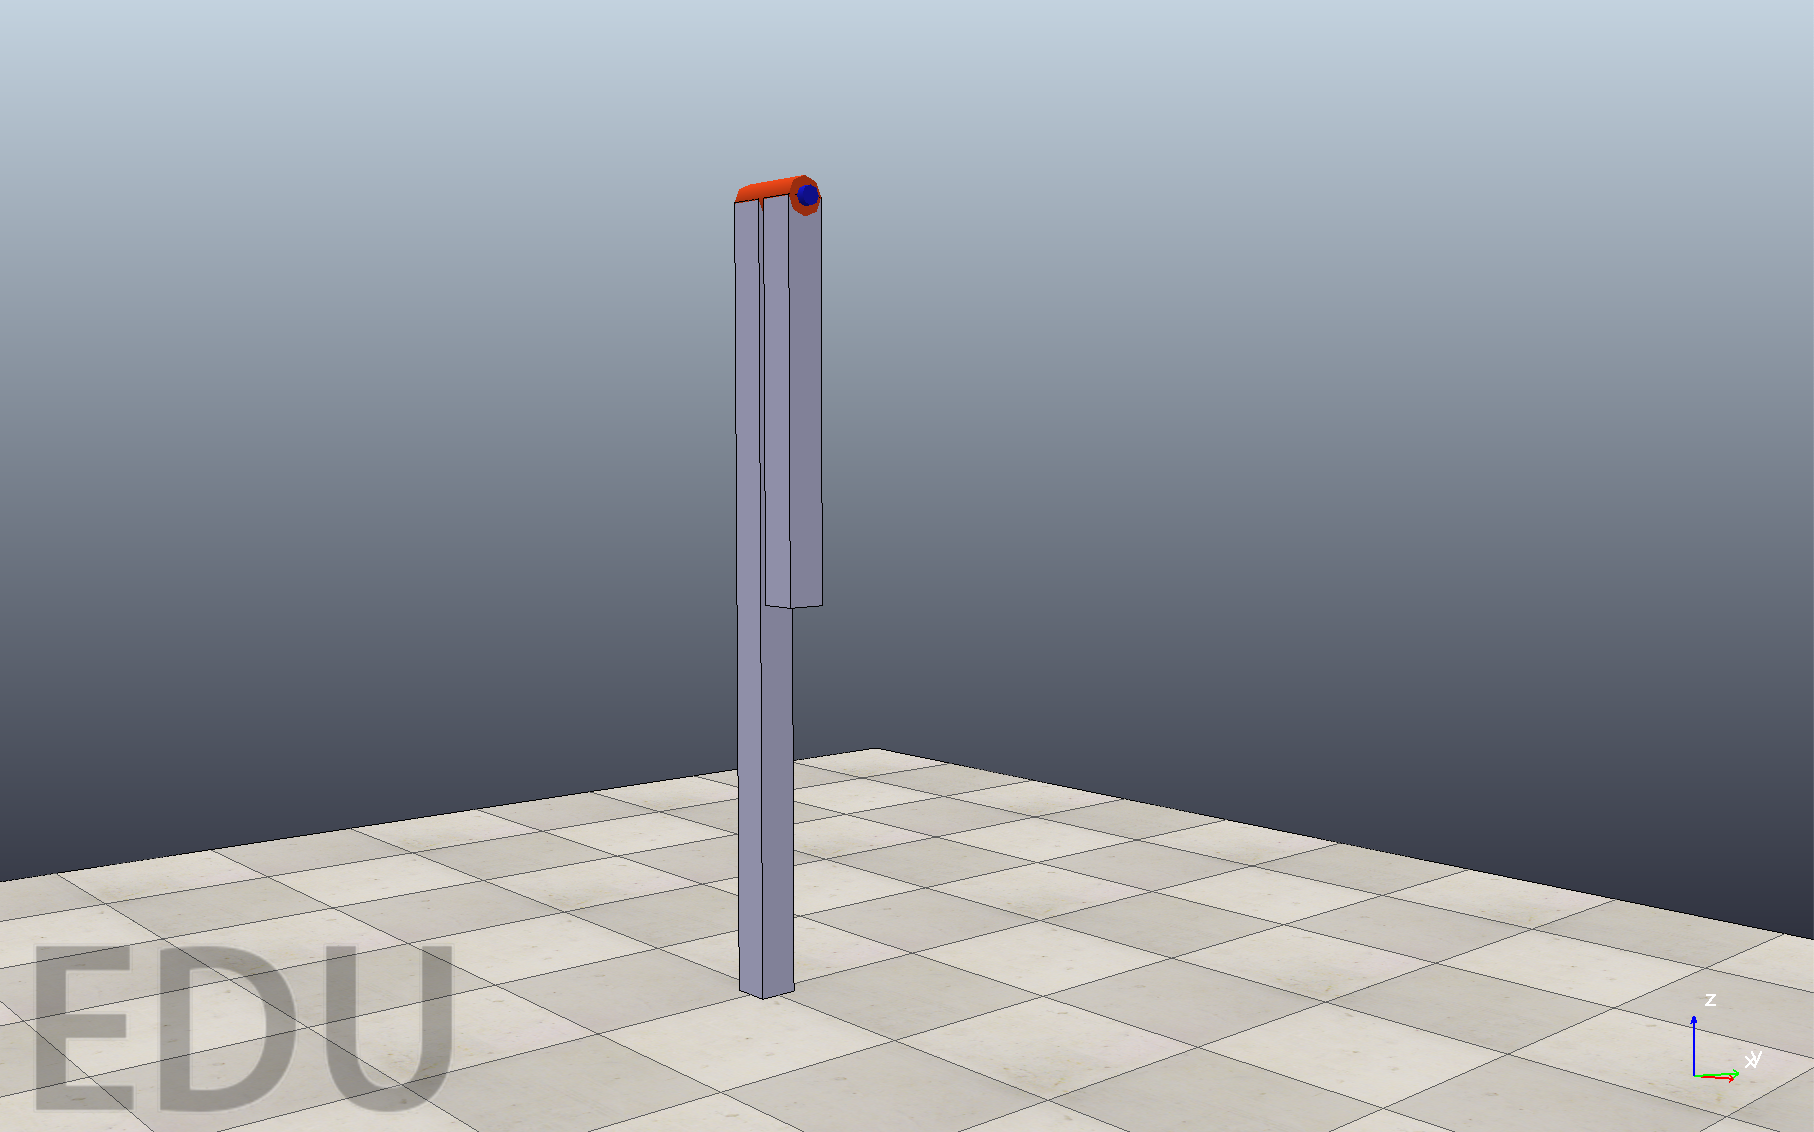
\includegraphics[width=0.7\textwidth]{images/1-dof/scene.png}
\caption{V-REP scene of the 1-dof robot arm}
\end{figure}
\FloatBarrier
The dynamic model of this kind of robot is:
\[u=gmd \sin(q) + (I+md^2)\ddot{q}= \begin{bmatrix}
\sin(q) & \ddot{q}
\end{bmatrix}\begin{bmatrix}
gmd \\ I +md^2
\end{bmatrix}\]
\begin{figure}[!htbp]
\centering
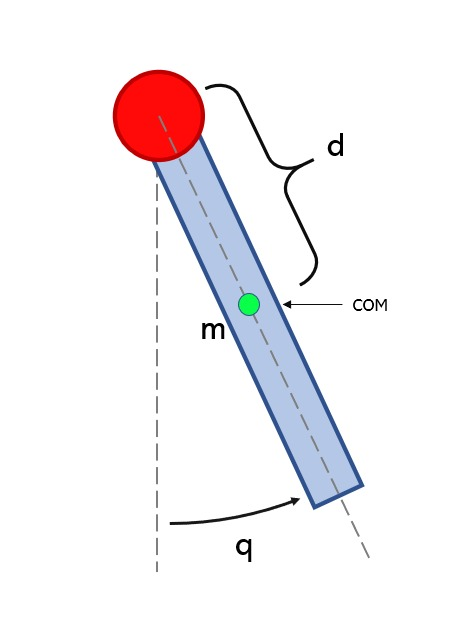
\includegraphics[width=0.4\textwidth]{images/1-dof/model.jpeg}
\caption{Robot arm model: $m$ is the mass of the link, $d$ is the position of the center of mass, $I$ is the moment of inertia when rotating around the center of mass}
\end{figure}
\FloatBarrier
Regarding the simulation, we have written a Matlab script in which we first connect to V-REP and then load the scene.\\
We generate exciting trajectories according to the following formula:
\[q_j(t) = \sum_{l=1}^{L}{\frac{ a_{l,j}}{ l\omega_f }\sin(l\omega_f t)-\frac{ b_{l,j}}{l\omega_f}\cos(l\omega_f t)+q_{0,j}}\]
We implemented a function called generate\_exciting\_traj() that generates a random exciting trajectory using the following parameters: $L = 5$ and $\omega_f = 0.1\pi$.
\\\\
After generated a trajectory, the simulation starts. In the main control loop we first get the joint position, velocity and torque (with –); then, we set a new target position according to the trajectory and the current instant of time.
\\\\
We obtain the measured accelerations through numerical differentiation; this leads to somewhat noisy values. In order to compensate for this noise, we apply a low-pass filter of order 16 and cutoff frequency equal to $0.35\pi$. Also the measured torques are noisy, so we apply the same filter.
\paragraph{}After that, we have all the ingredients to generate the regressor matrix with all the computed values by staking all the $Y$ in a unique matrix. We do the same for the measured torques obtaining a vector $\overline{\tau}$.

\subsection{Experiments}
\paragraph{}We have generated four trajectories made by the combination of sines and cosines through the generate\_exciting\_traj() function. \\ All these trajectories are repeated 5 consecutive times but we take only the 3 intermediate periods. The results are reported below.
\pagebreak

\paragraph{Experiment 1}
We report the results of the simulation with the first trajectory generated:
\begin{figure}[!htbp]
\centering
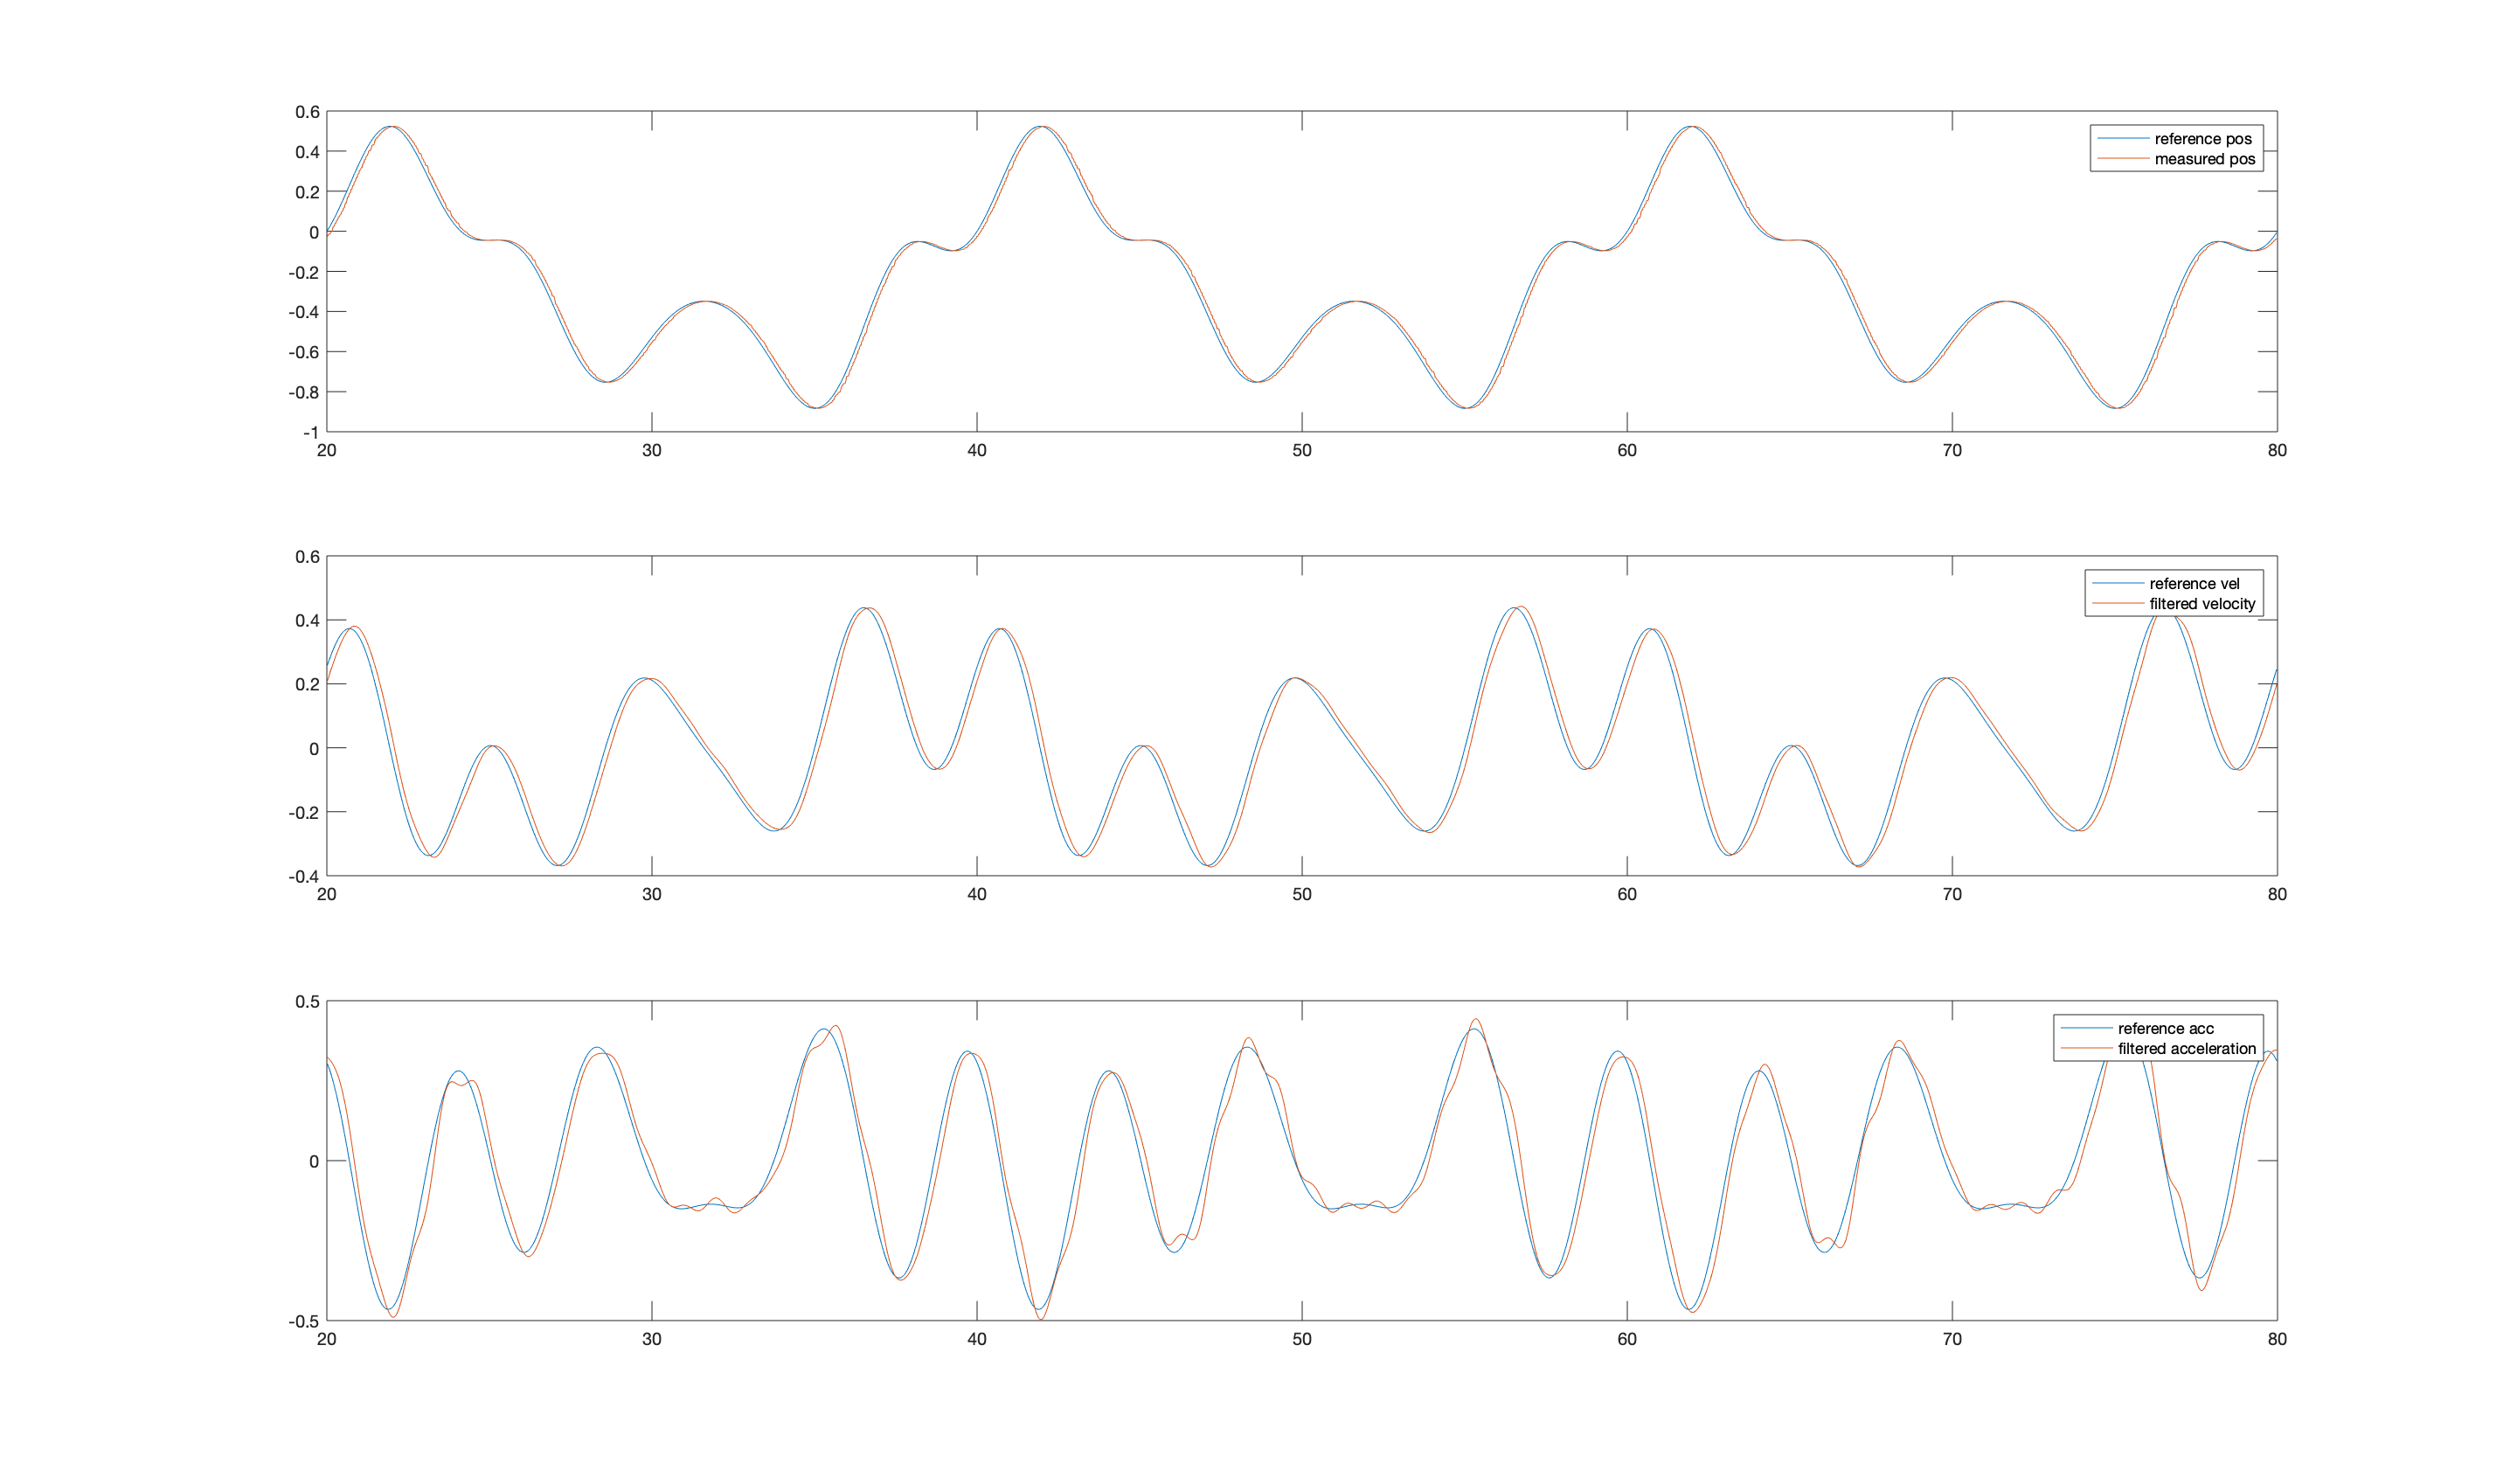
\includegraphics[width=0.7\textwidth]{images/1-dof/experiment1_traj.png}
\caption{Plot of the reference position, velocity and acceleration vs measured position, velocity and (filtered) acceleration}
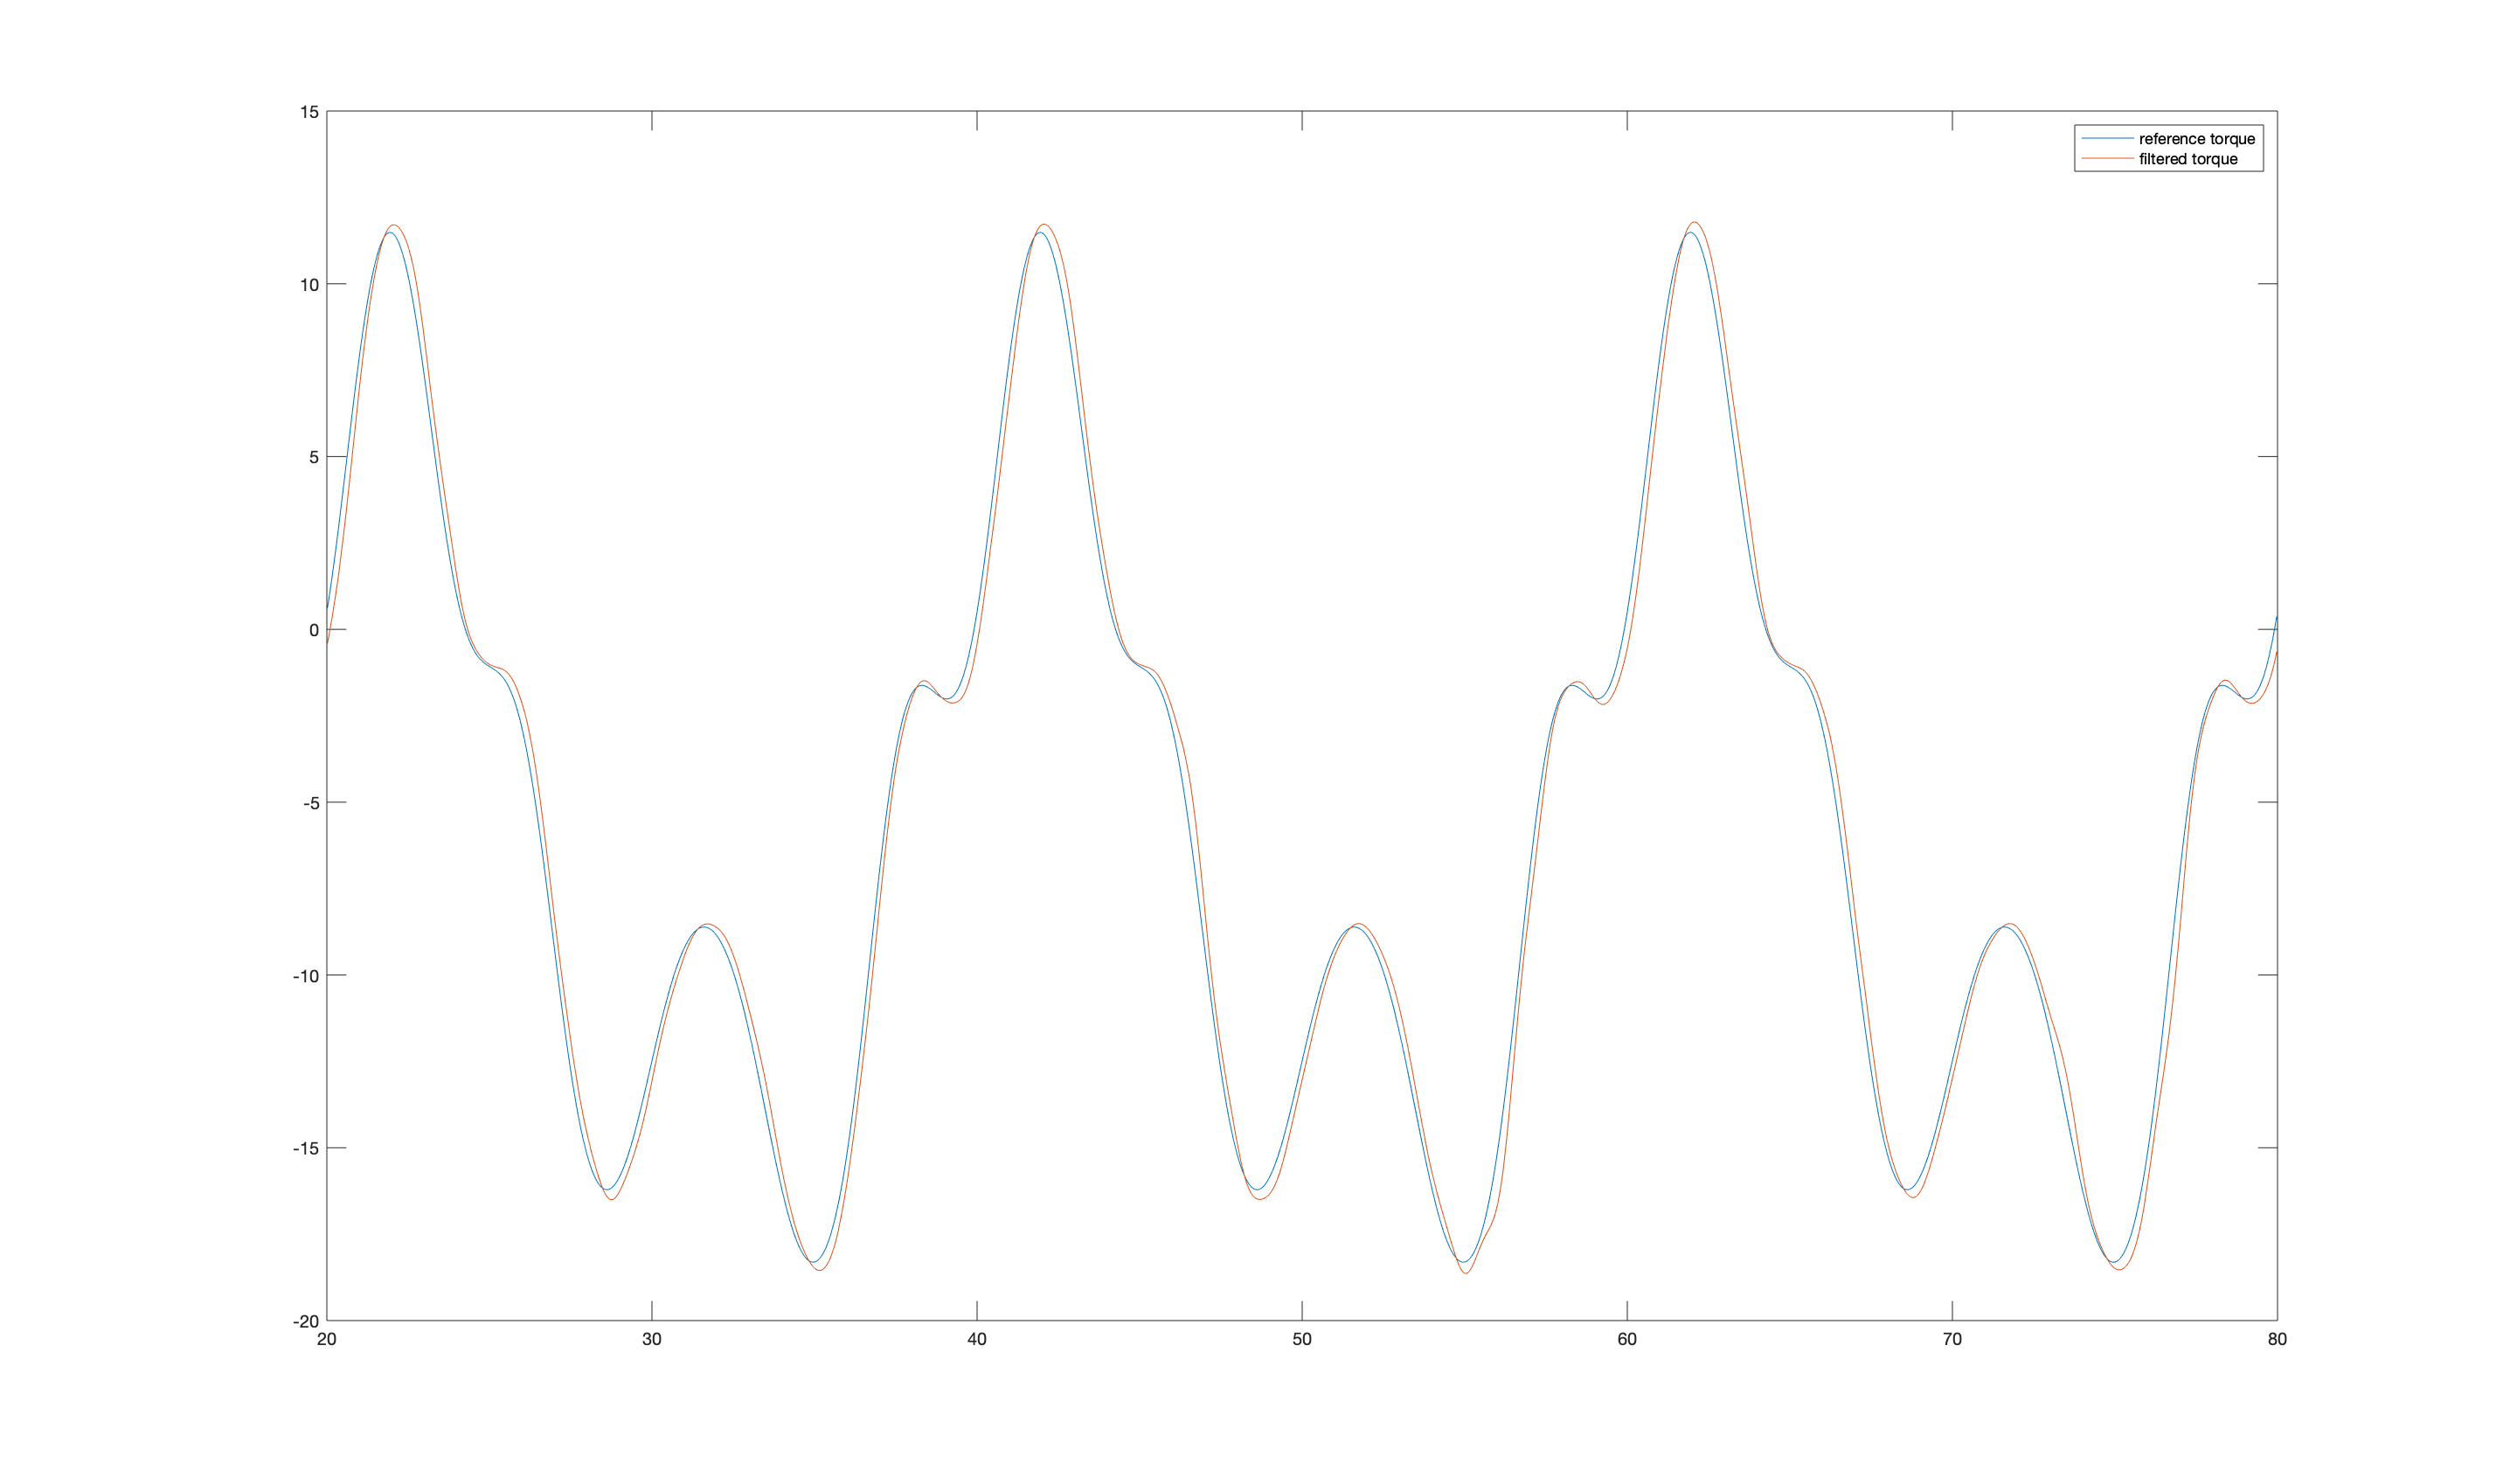
\includegraphics[width=0.7\textwidth]{images/1-dof/experiment1.png}
\caption{Plot of the reference torque computed using the dynamic model and the reference position, velocity and acceleration vs (filtered) measured torque}
\end{figure}
\pagebreak

\paragraph{Experiment 2}
We report the results of the simulation with the second trajectory generated:
\begin{figure}[!htbp]
\centering
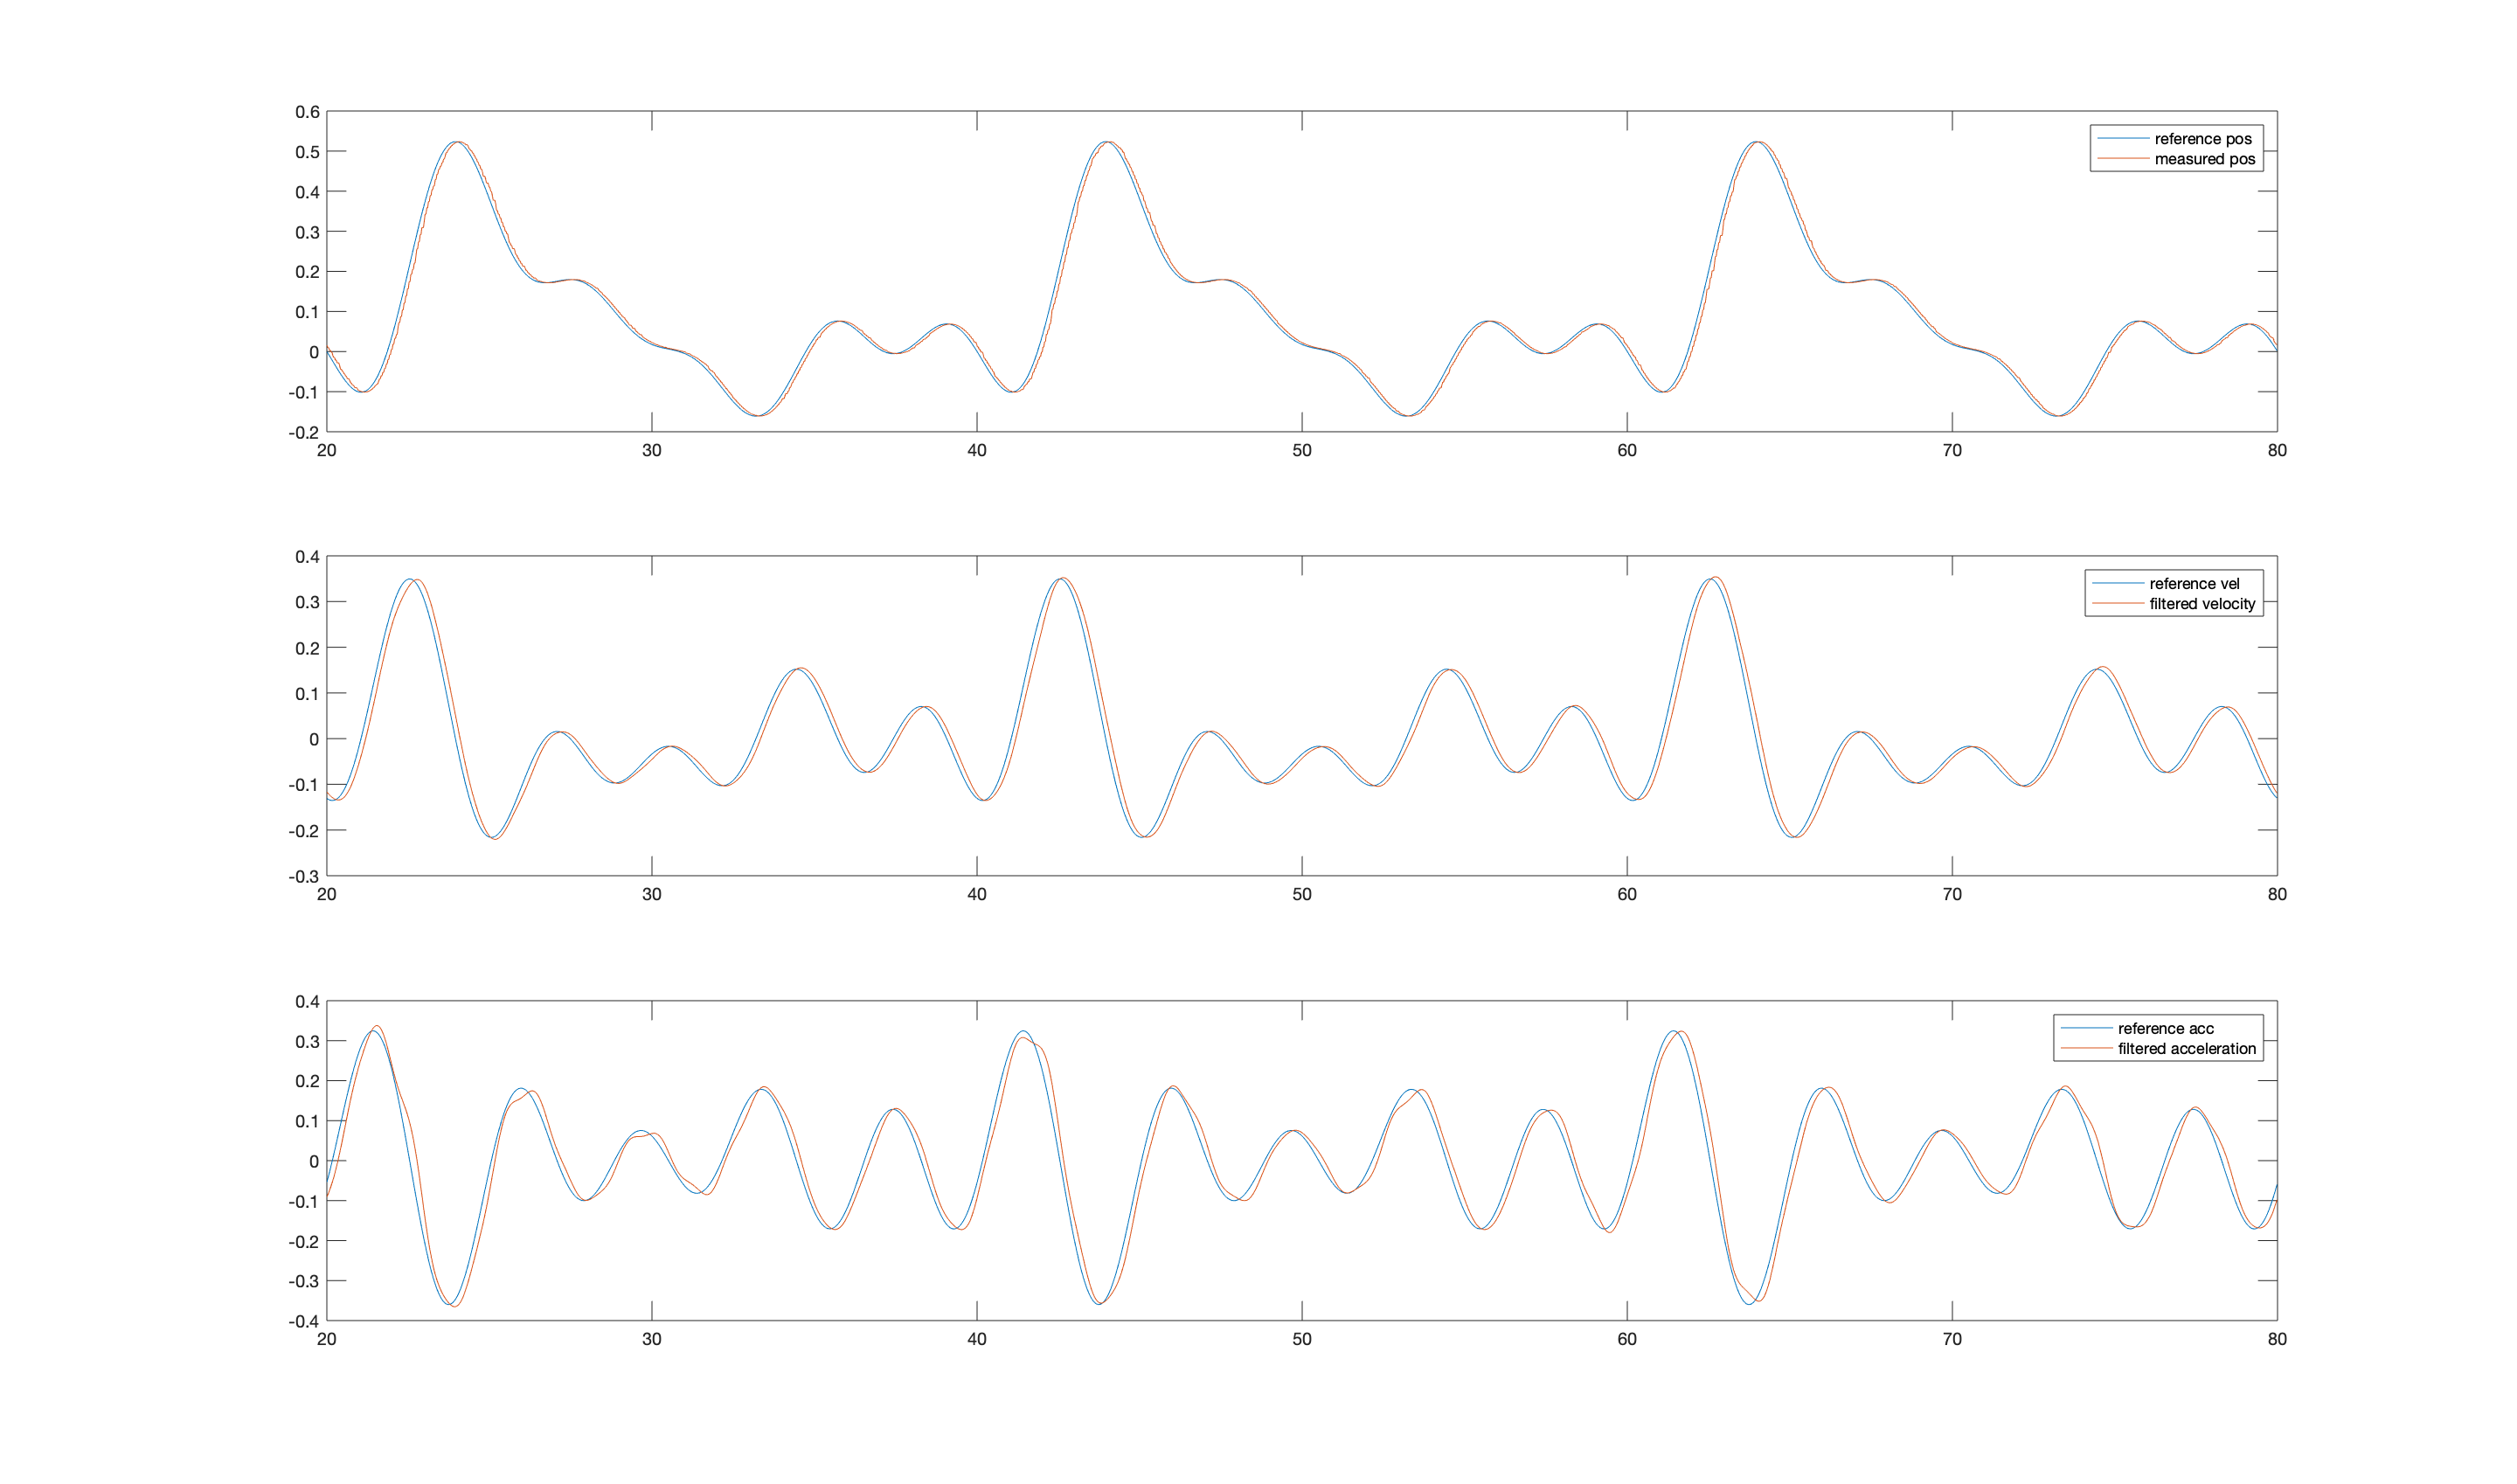
\includegraphics[width=0.7\textwidth]{images/1-dof/experiment2_traj.png}
\caption{Plot of the reference position, velocity and acceleration vs measured position, velocity and (filtered) acceleration}
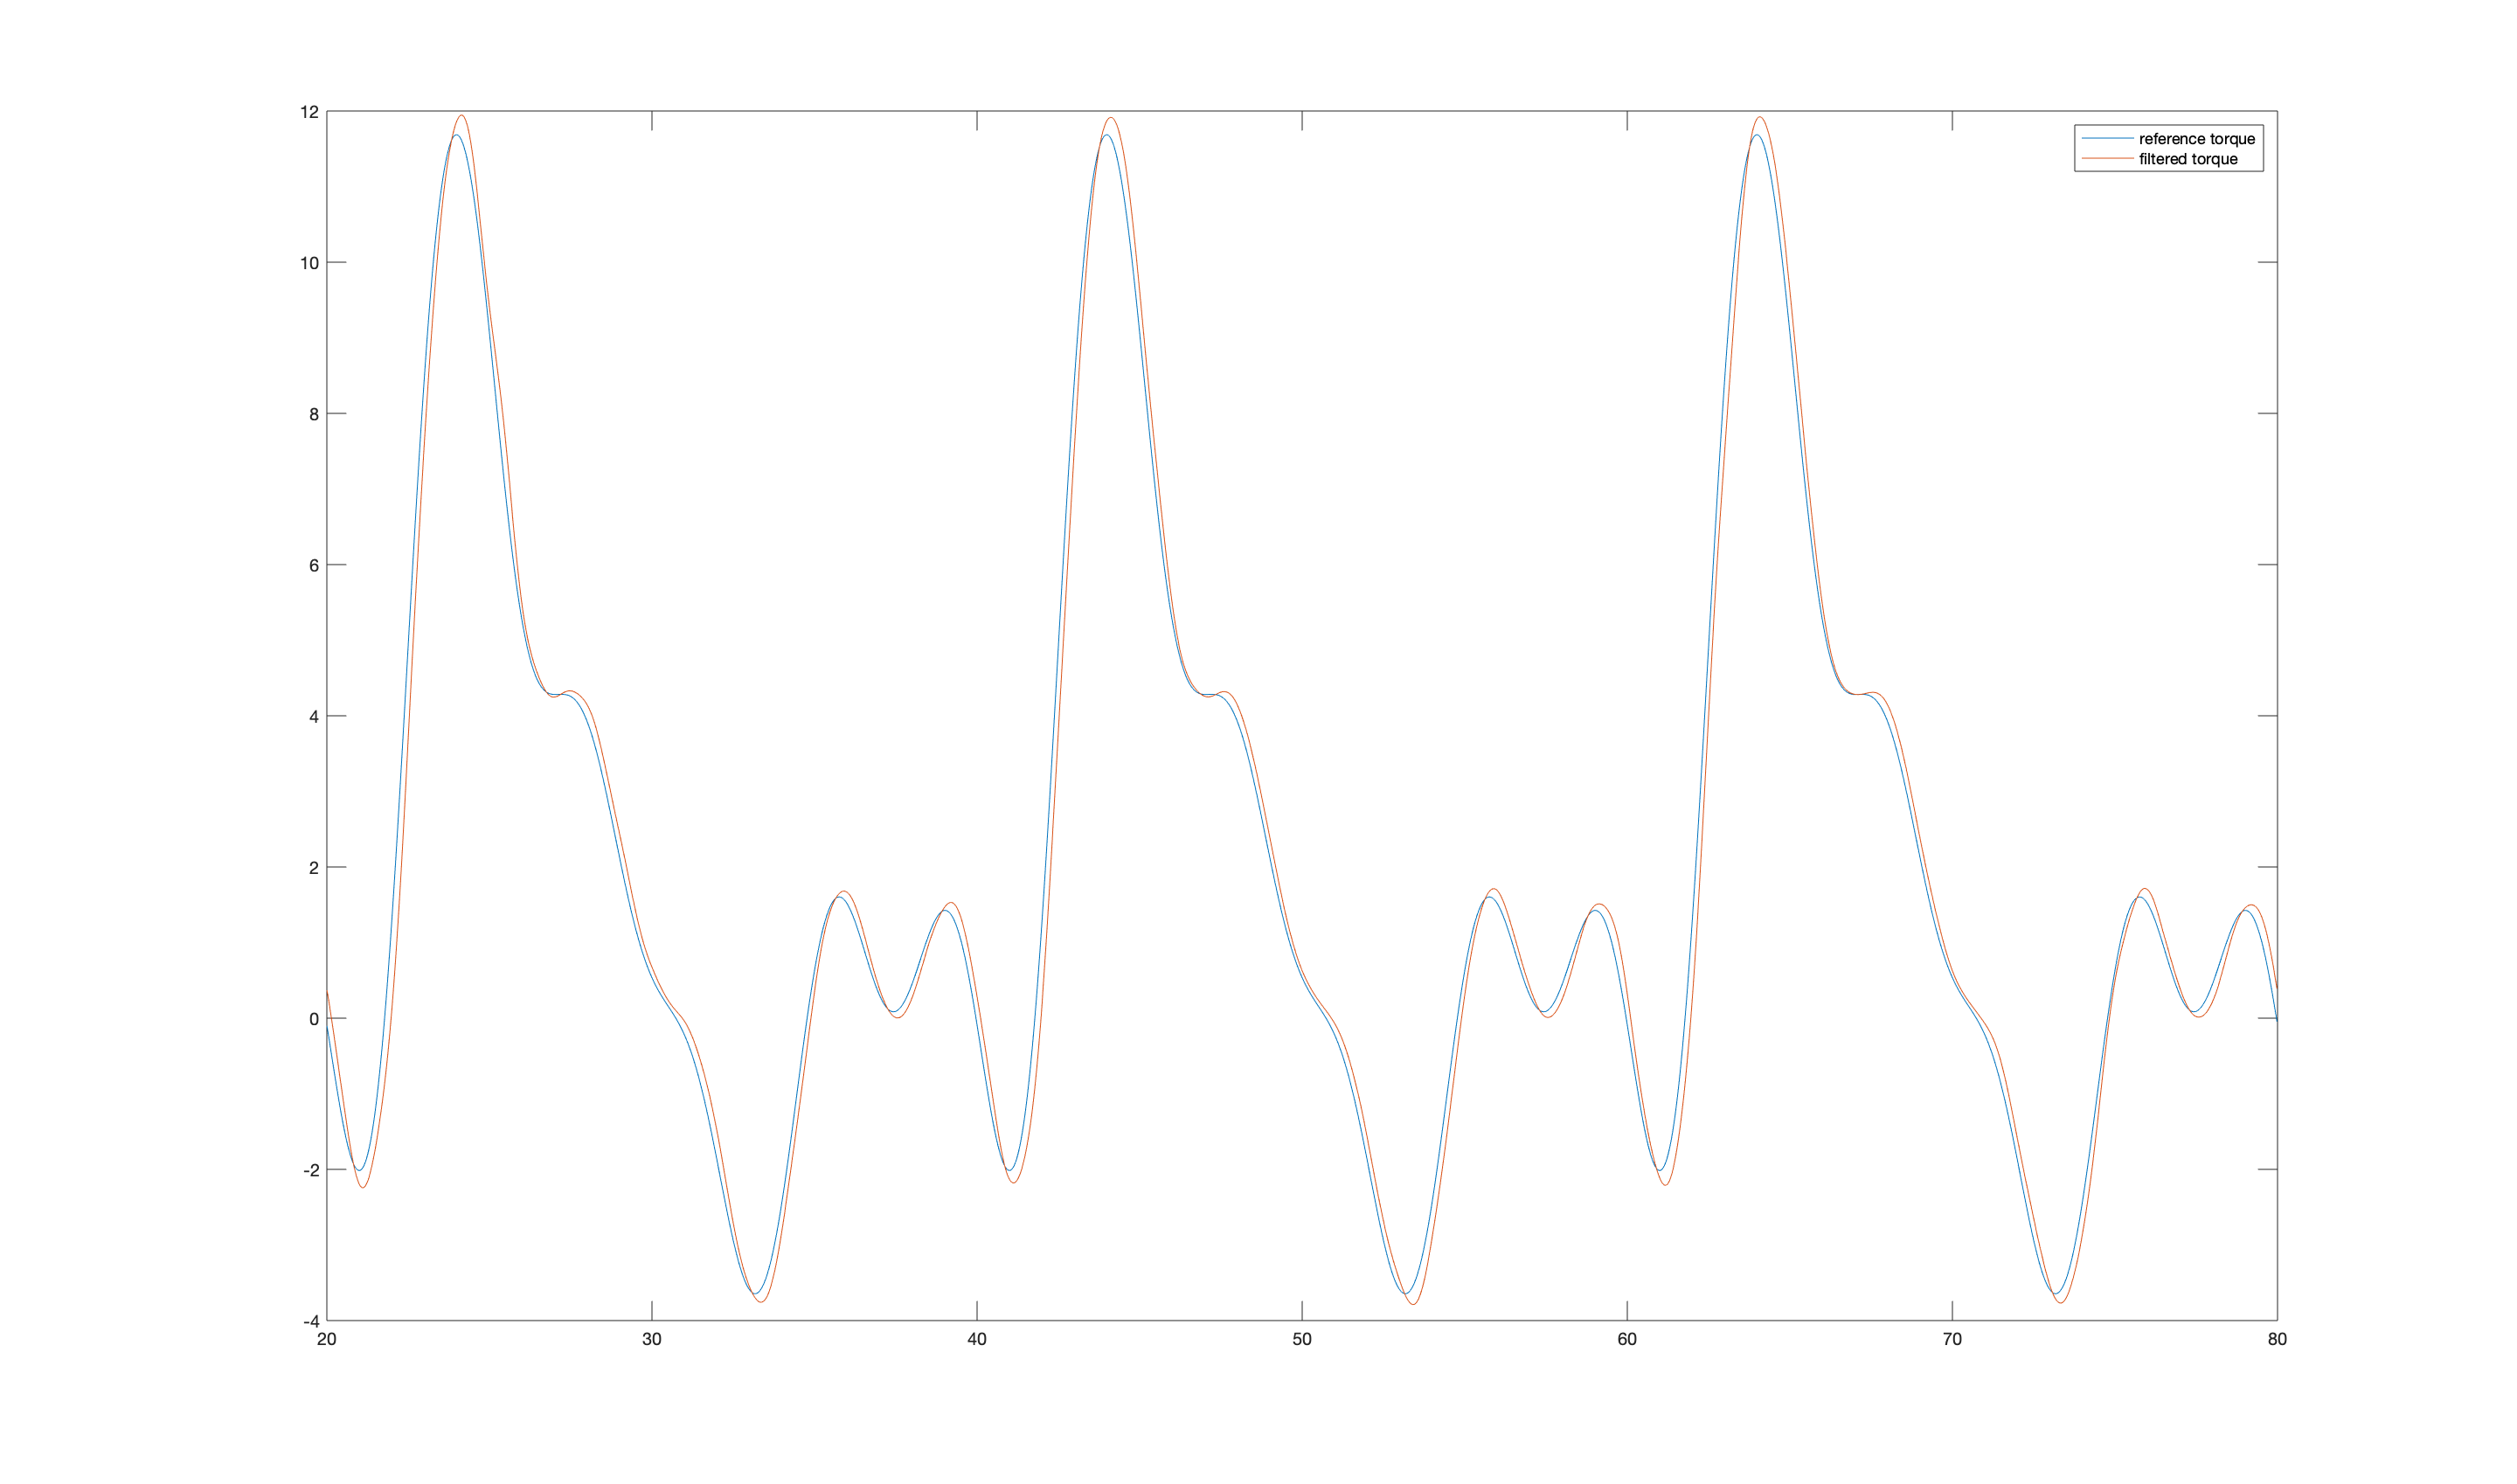
\includegraphics[width=0.7\textwidth]{images/1-dof/experiment2.png}
\caption{Plot of the reference torque computed using the dynamic model and the reference position, velocity and acceleration vs (filtered) measured torque}
\end{figure}
\pagebreak

\paragraph{Experiment 3}
We report the results of the simulation with the third trajectory generated:
\begin{figure}[!htbp]
\centering
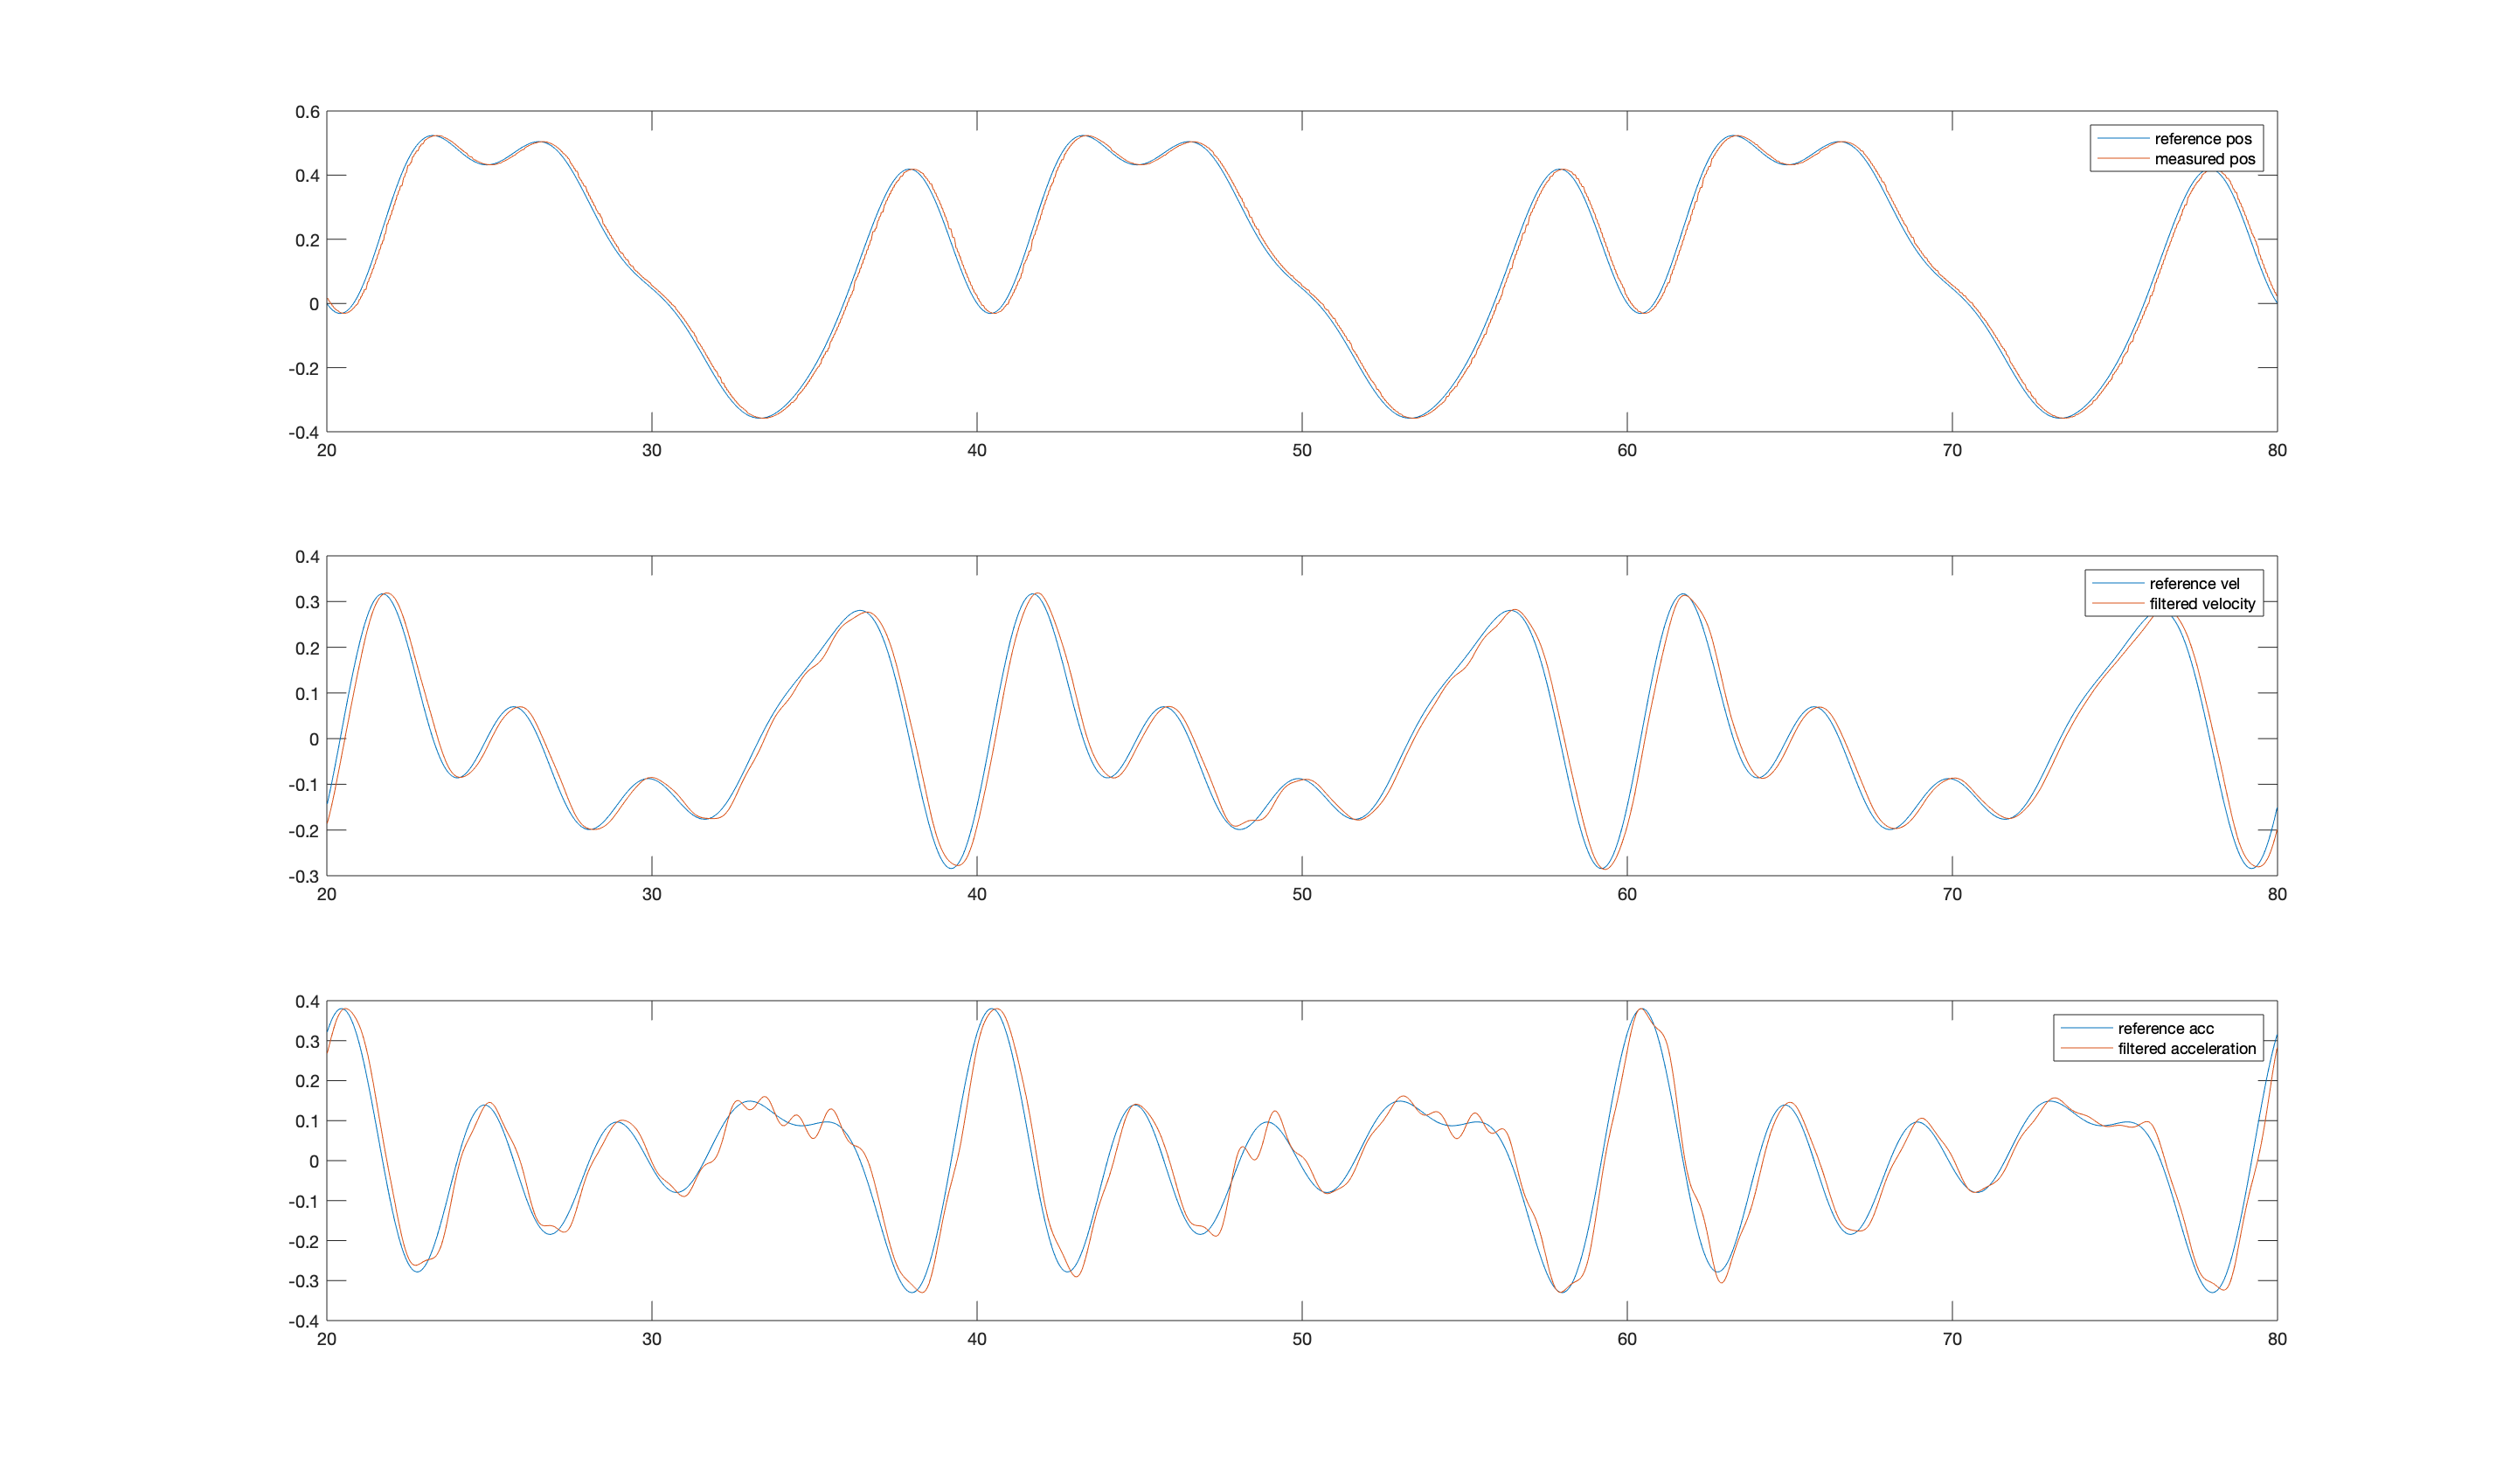
\includegraphics[width=0.7\textwidth]{images/1-dof/experiment3_traj.png}
\caption{Plot of the reference position, velocity and acceleration vs measured position, velocity and (filtered) acceleration}
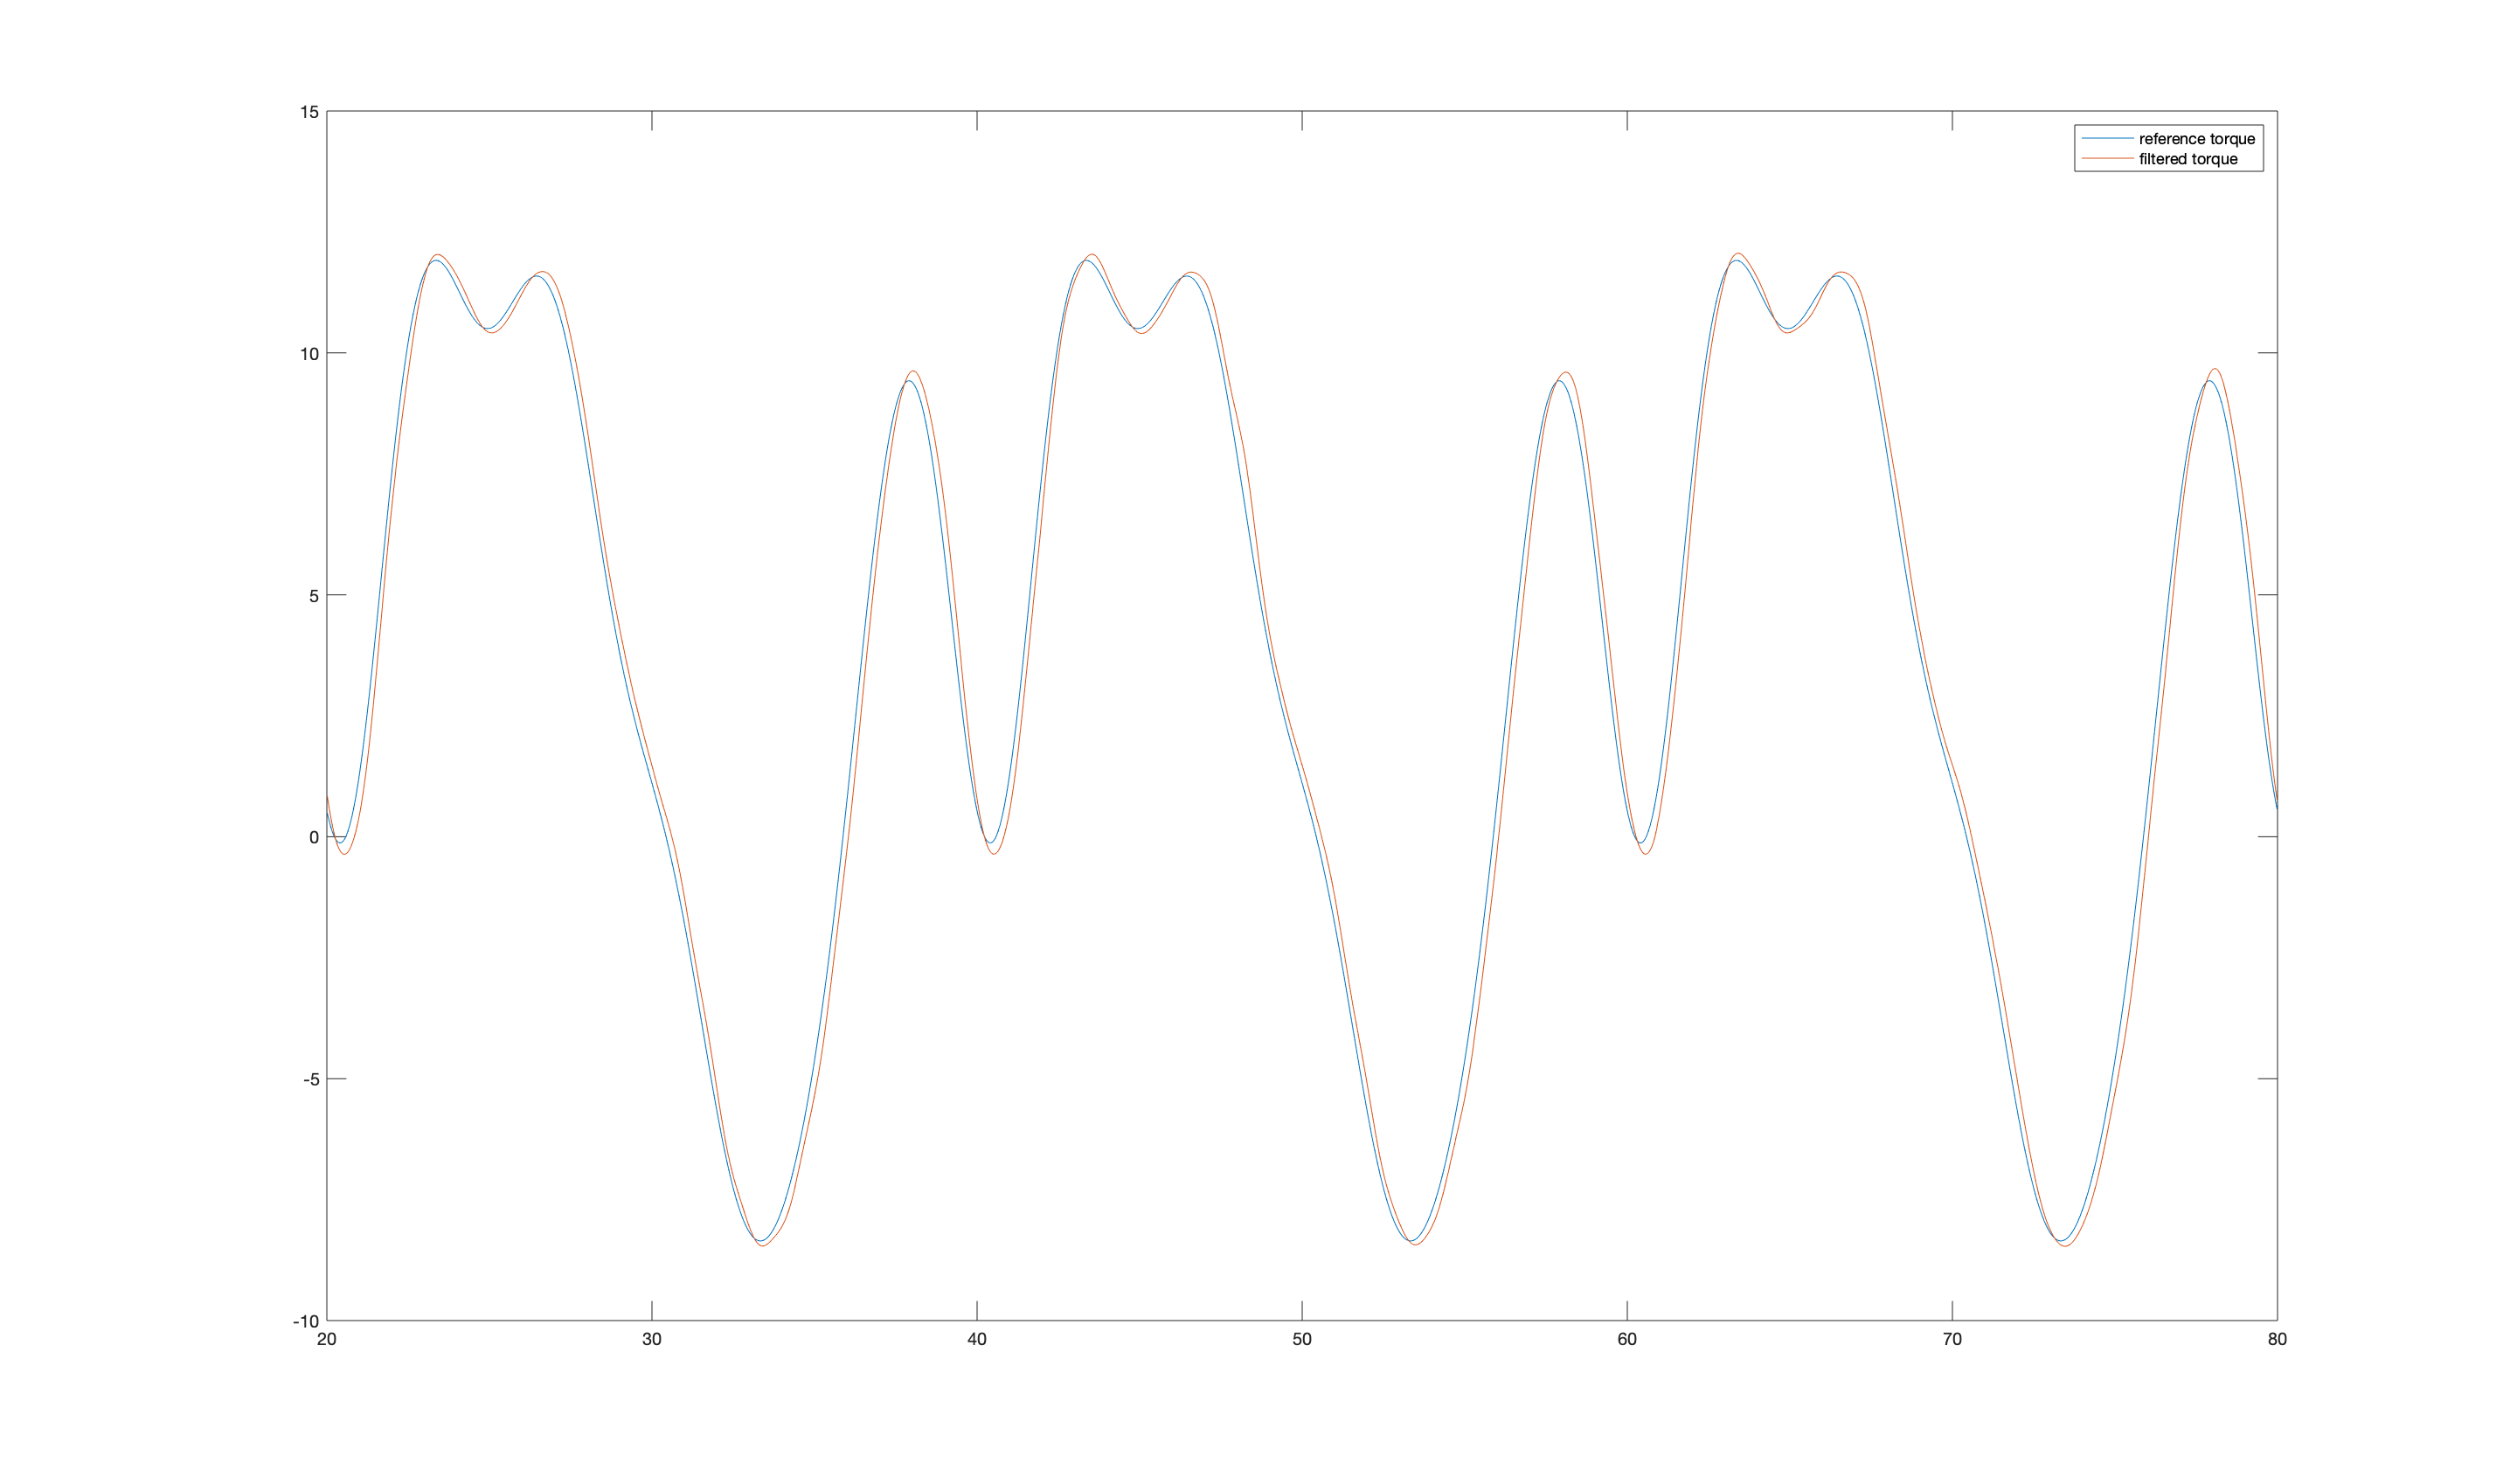
\includegraphics[width=0.7\textwidth]{images/1-dof/experiment3.png}
\caption{Plot of the reference torque computed using the dynamic model and the reference position, velocity and acceleration vs (filtered) measured torque}
\end{figure}
\pagebreak

\paragraph{Experiment 4}
We report the results of the simulation with the fourth trajectory generated:
\begin{figure}[!htbp]
\centering
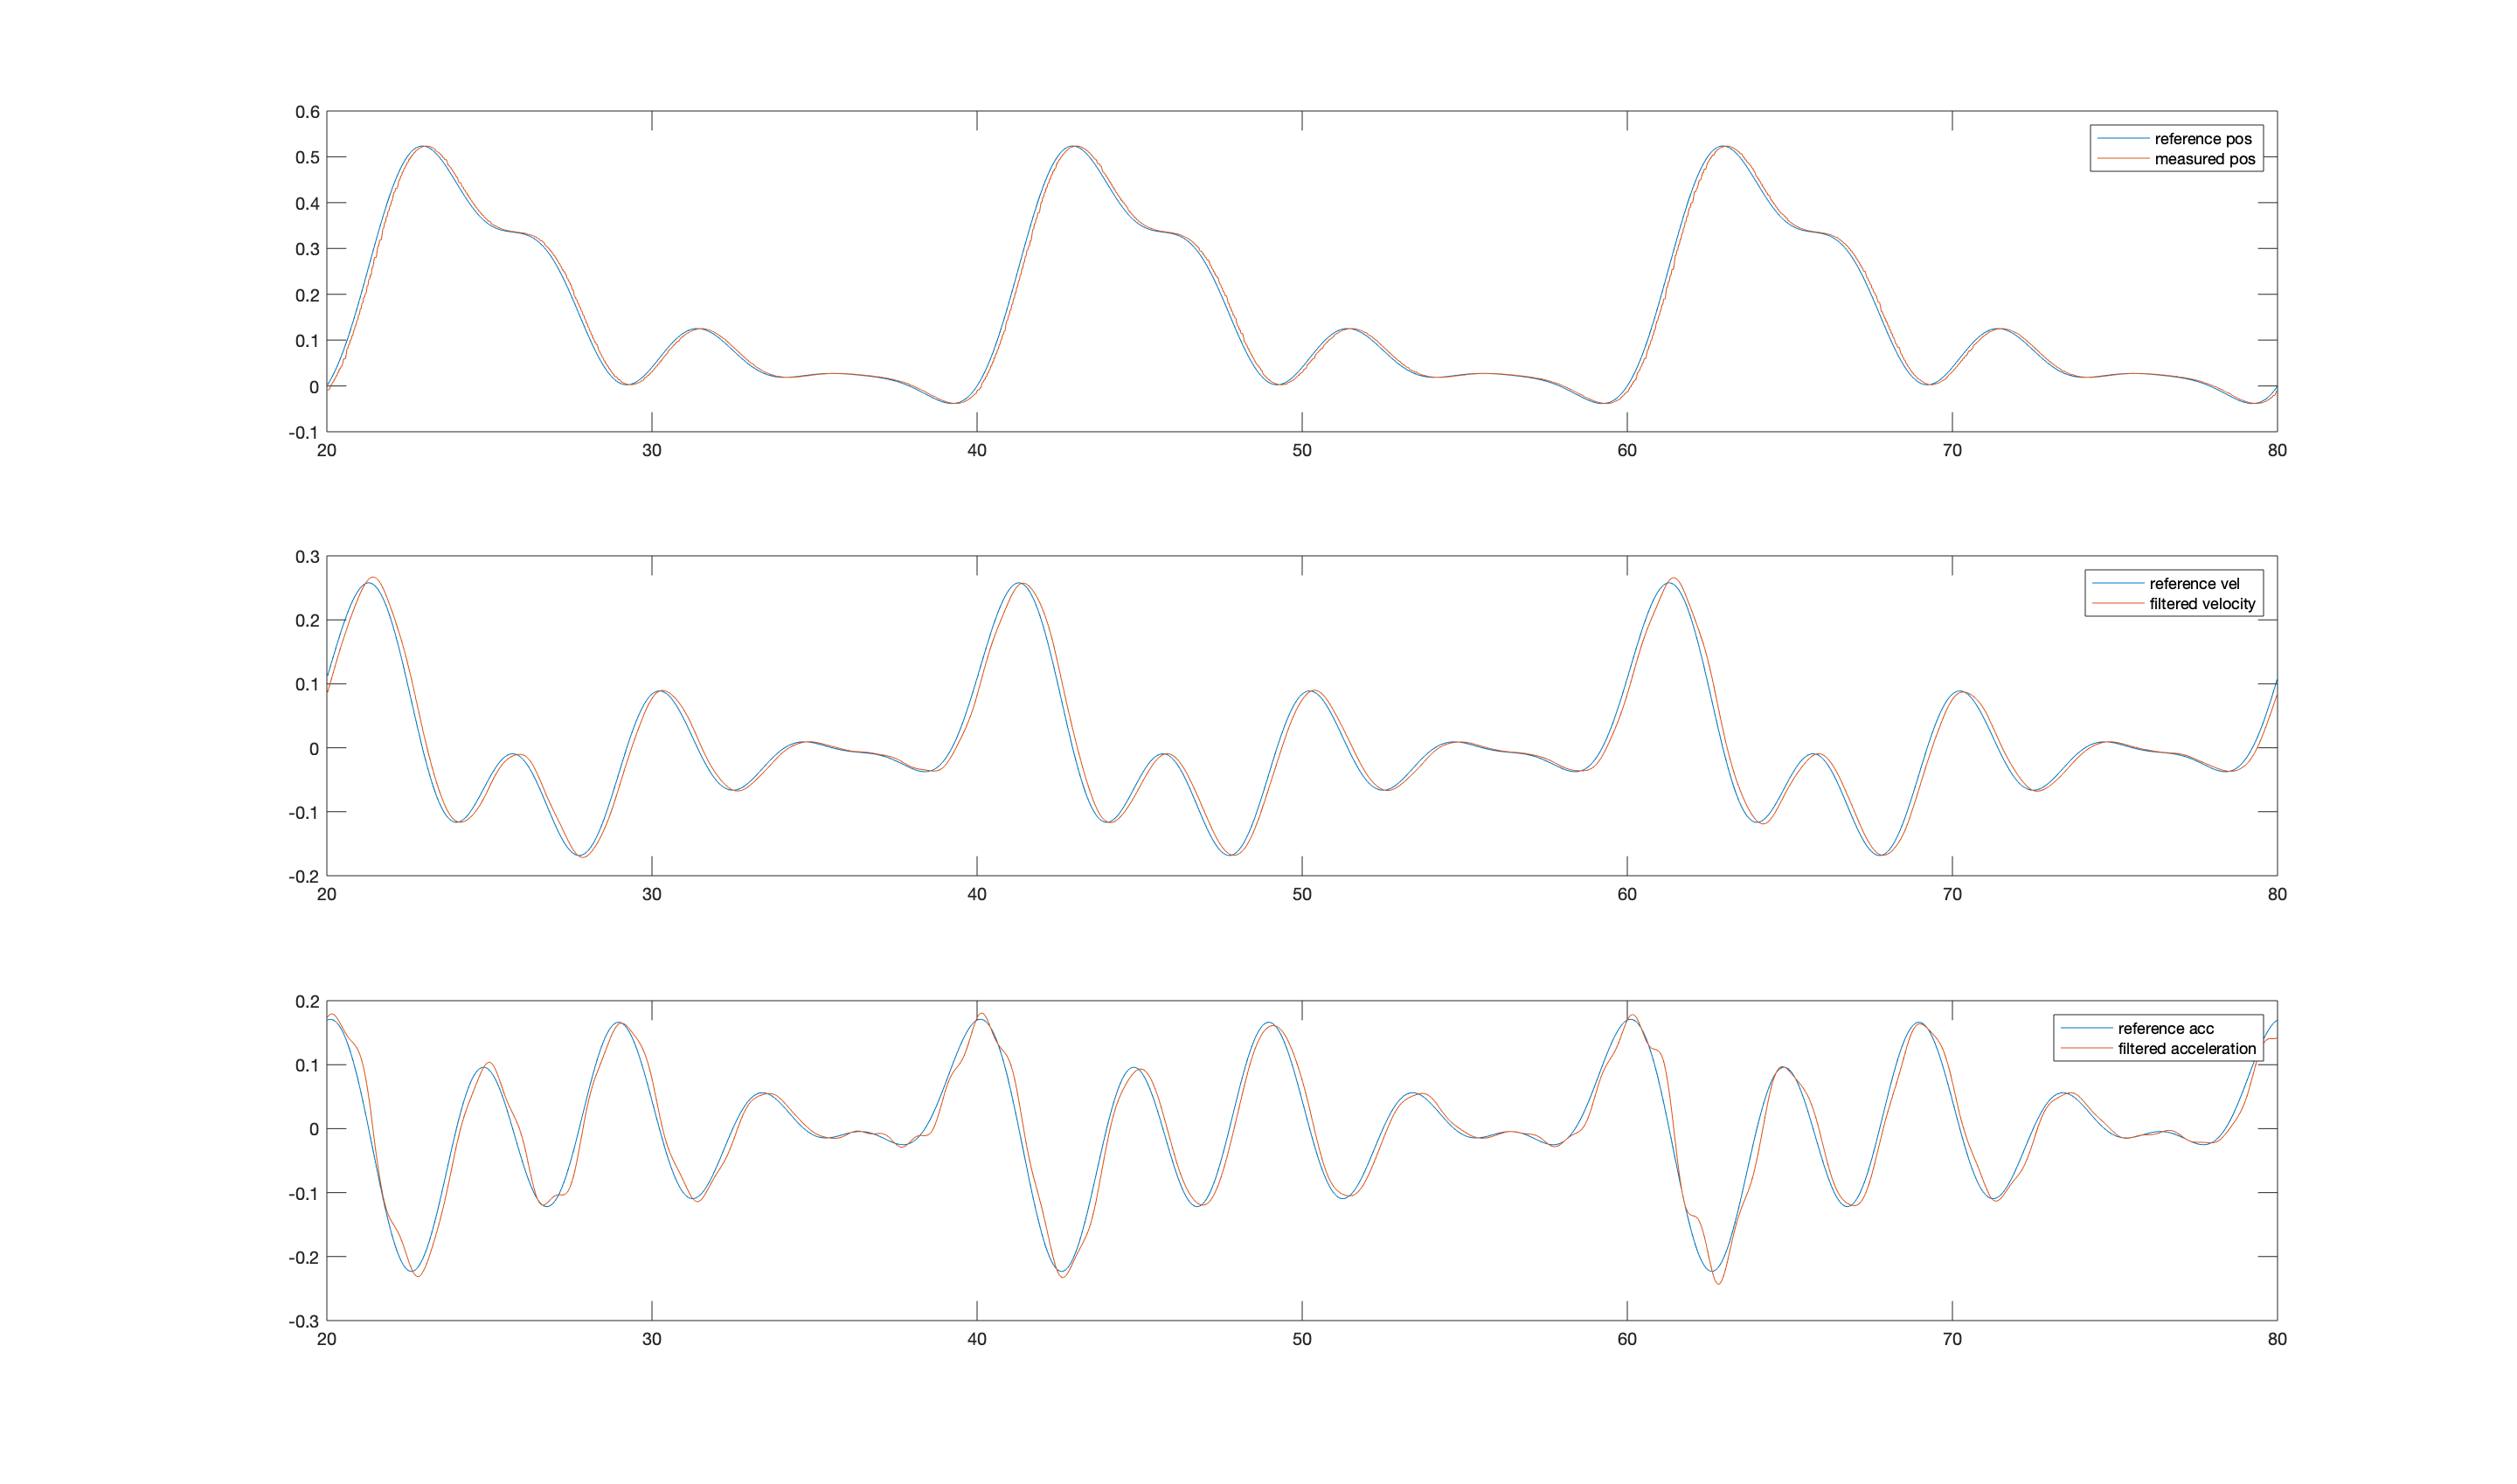
\includegraphics[width=0.7\textwidth]{images/1-dof/experiment4_traj.png}
\caption{Plot of the reference position, velocity and acceleration vs measured position, velocity and (filtered) acceleration}
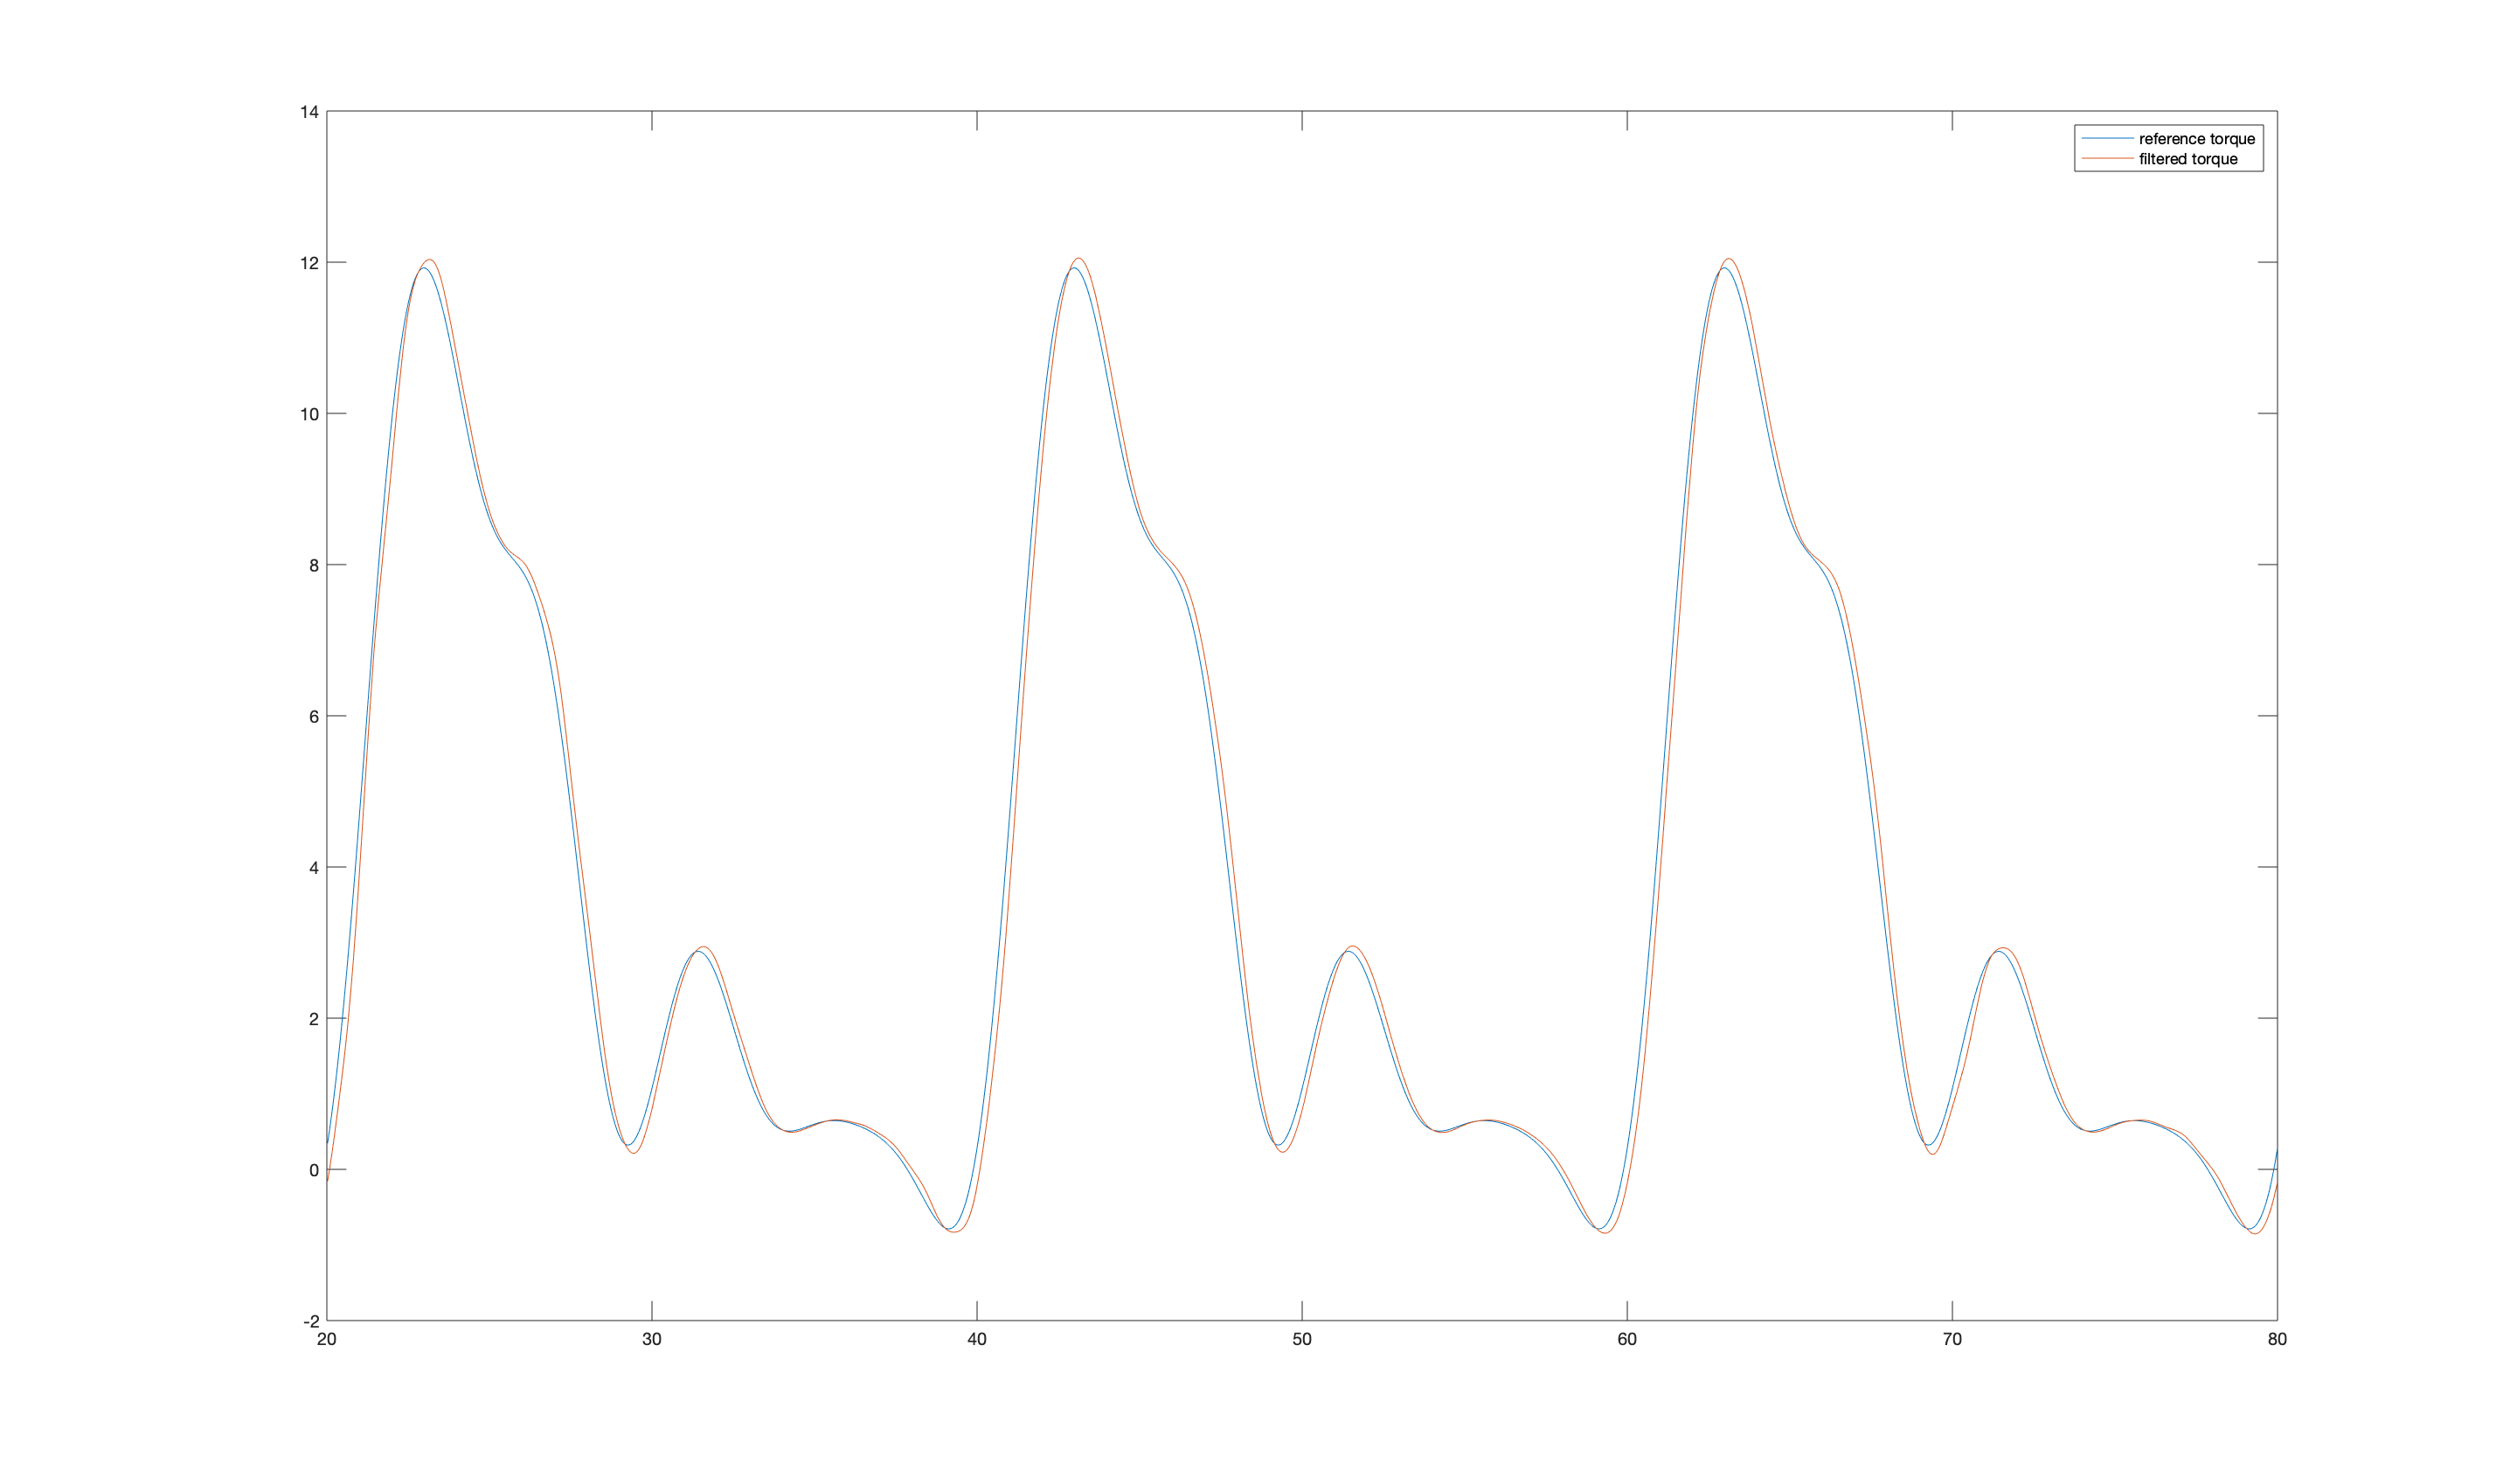
\includegraphics[width=0.7\textwidth]{images/1-dof/experiment4.png}
\caption{Plot of the reference torque computed using the dynamic model and the reference position, velocity and acceleration vs (filtered) measured torque}
\end{figure}
\pagebreak

\subsection{PBRP algorithm}
\paragraph{}If we had torque signs, we would apply directly the Penalty-Based Parameters Retrivial (PBRP) algorithm. The aim of this algorithm is to get a physically consistent set of parameters; in order to do so, we need to solve the following optimization problem:
\[\min_{p_k}{\phi(p_k)} = \lVert \overline{Y}\pi(p_k)-\overline{\tau} \rVert^2\]

\noindent where $\overline{Y}$ is the stacked regressor, $\overline{\tau}$ is the stacked  torque measurements and $\pi(p_k)$ is the coefficients vector computed from the current parameters vector $p_k$.

\paragraph{}In order to obtain a physically consistent set of parameters, we should put constraints on the mass and on the inertia. Since we are dealing with a 1 dof robot, the only constraints we have is that both mass and inertia should be positive.

\[m > 0, I > 0\]

In general, it is possible to provide a set of lower and upper bounds for the dynamic parameters based on a priori knowledge. For instance, the center of mass must be inside the convex link of the robot. However, the aim of our work is to estimate the dynamic coefficients without torque signs. So, we cannot apply this algorithm directly, but we need a preliminary analysis in which we predict what is the most likely torque sign.

\subsection{Tree of solutions}
\paragraph{}First of all, we take the absolute values of the filtered measured torques. Then, we have to "mark" the function whenever it crosses 0. In order to do this, we should tolerate a threshold; we compute this threshold by discarding the 10\% of samples closer to 0. At this point, we discard all the samples under threshold; we are left with several segments so that in each of them the sign of the torque is either positive or negative.
\paragraph{}After that, we have to predict the torque sign for each segment. The idea is: we first take a random segment which could be either positive or negative, so we have two possible solutions; then, we take another segment which again could be either positive or negative, so at this stage we have four possible solutions (by considering the previous ones), and so on. This is an exponential problem, so if we have $n$ segments we would have $2^n$ possible solutions. However, it is possible to prevent the tree from being completely expanded because we can recognize in advance when a choice of sign lead to a wrong solution; in fact, when the PBRP algorithm is applied to a torque with the wrong sign, the loss should be higher than the one with the correct sign. So, at each level of the tree, we expand only the best nodes which are the ones with the lower loss until that segments (in our case, we decided to expand the best 5 nodes). For all the optimization problems of the tree we use pattern search algorithm because it is faster.
\paragraph{}At the end of this tree algorithm, we will obtain the best combination of signs for the segments sequence. So, we apply the PBRP algorithm to this sequence with a number of runs equal to 3 using simulated annealing.

\subsection{Results}
\paragraph{}In this section we are going to show the results obtained by applying the PBRP algorithm to the torques with the estimated signs.

\begin{table}[!htbp]
\centering
\begin{tabular}{|c|ccc|}
\hline
& $m$ & $d$ & $I$\\
\hline
Ground truth & 5 & 0.5 & 0.4208\\
Experiment 1 & 6.1966 & 0.4035 & $3.9016\cdot 10^{-4}$\\
Experiment 2 & 7.1361 & 0.3488 & 0.0864\\
Experiment 3 & 7.3009 & 0.3428 & 0.1789\\
Experiment 4 & 6.1980 & 0.4036 & 0\\
\hline
\end{tabular}
\caption{Optimal solutions}
\end{table}

As we can see from the table, the optimal solutions that we get are quite different from the nominal values of the dynamic parameters. However, we are interested in the dynamic coefficients, so for each experiment, we will report the estimated dynamic coefficients compared with their ground values. In order to get a measure of the error, we decide to take the norm of the difference between these two vectors.

\paragraph{}We remember that:

\[\bm{\pi}= \begin{bmatrix}
\pi_1 \\ \pi_2
\end{bmatrix} = \begin{bmatrix}
gmd \\ I +md^2
\end{bmatrix}\]

The ground values of the dynamic coefficients are:

\[\begin{bmatrix}
\pi_1 \\ \pi_2
\end{bmatrix}=\begin{bmatrix}
24.5250 \\ 1.6708
\end{bmatrix}\]

\paragraph{Experiment 1} The estimated dynamic coefficients without torque signs are:

\[\begin{bmatrix}
\pi_1  \\ \pi_2 
\end{bmatrix}=\begin{bmatrix}
24.5288 \\ 1.0093
\end{bmatrix}\]

The norm of the error is 0.6615.

\begin{figure}[!htbp]
\centering
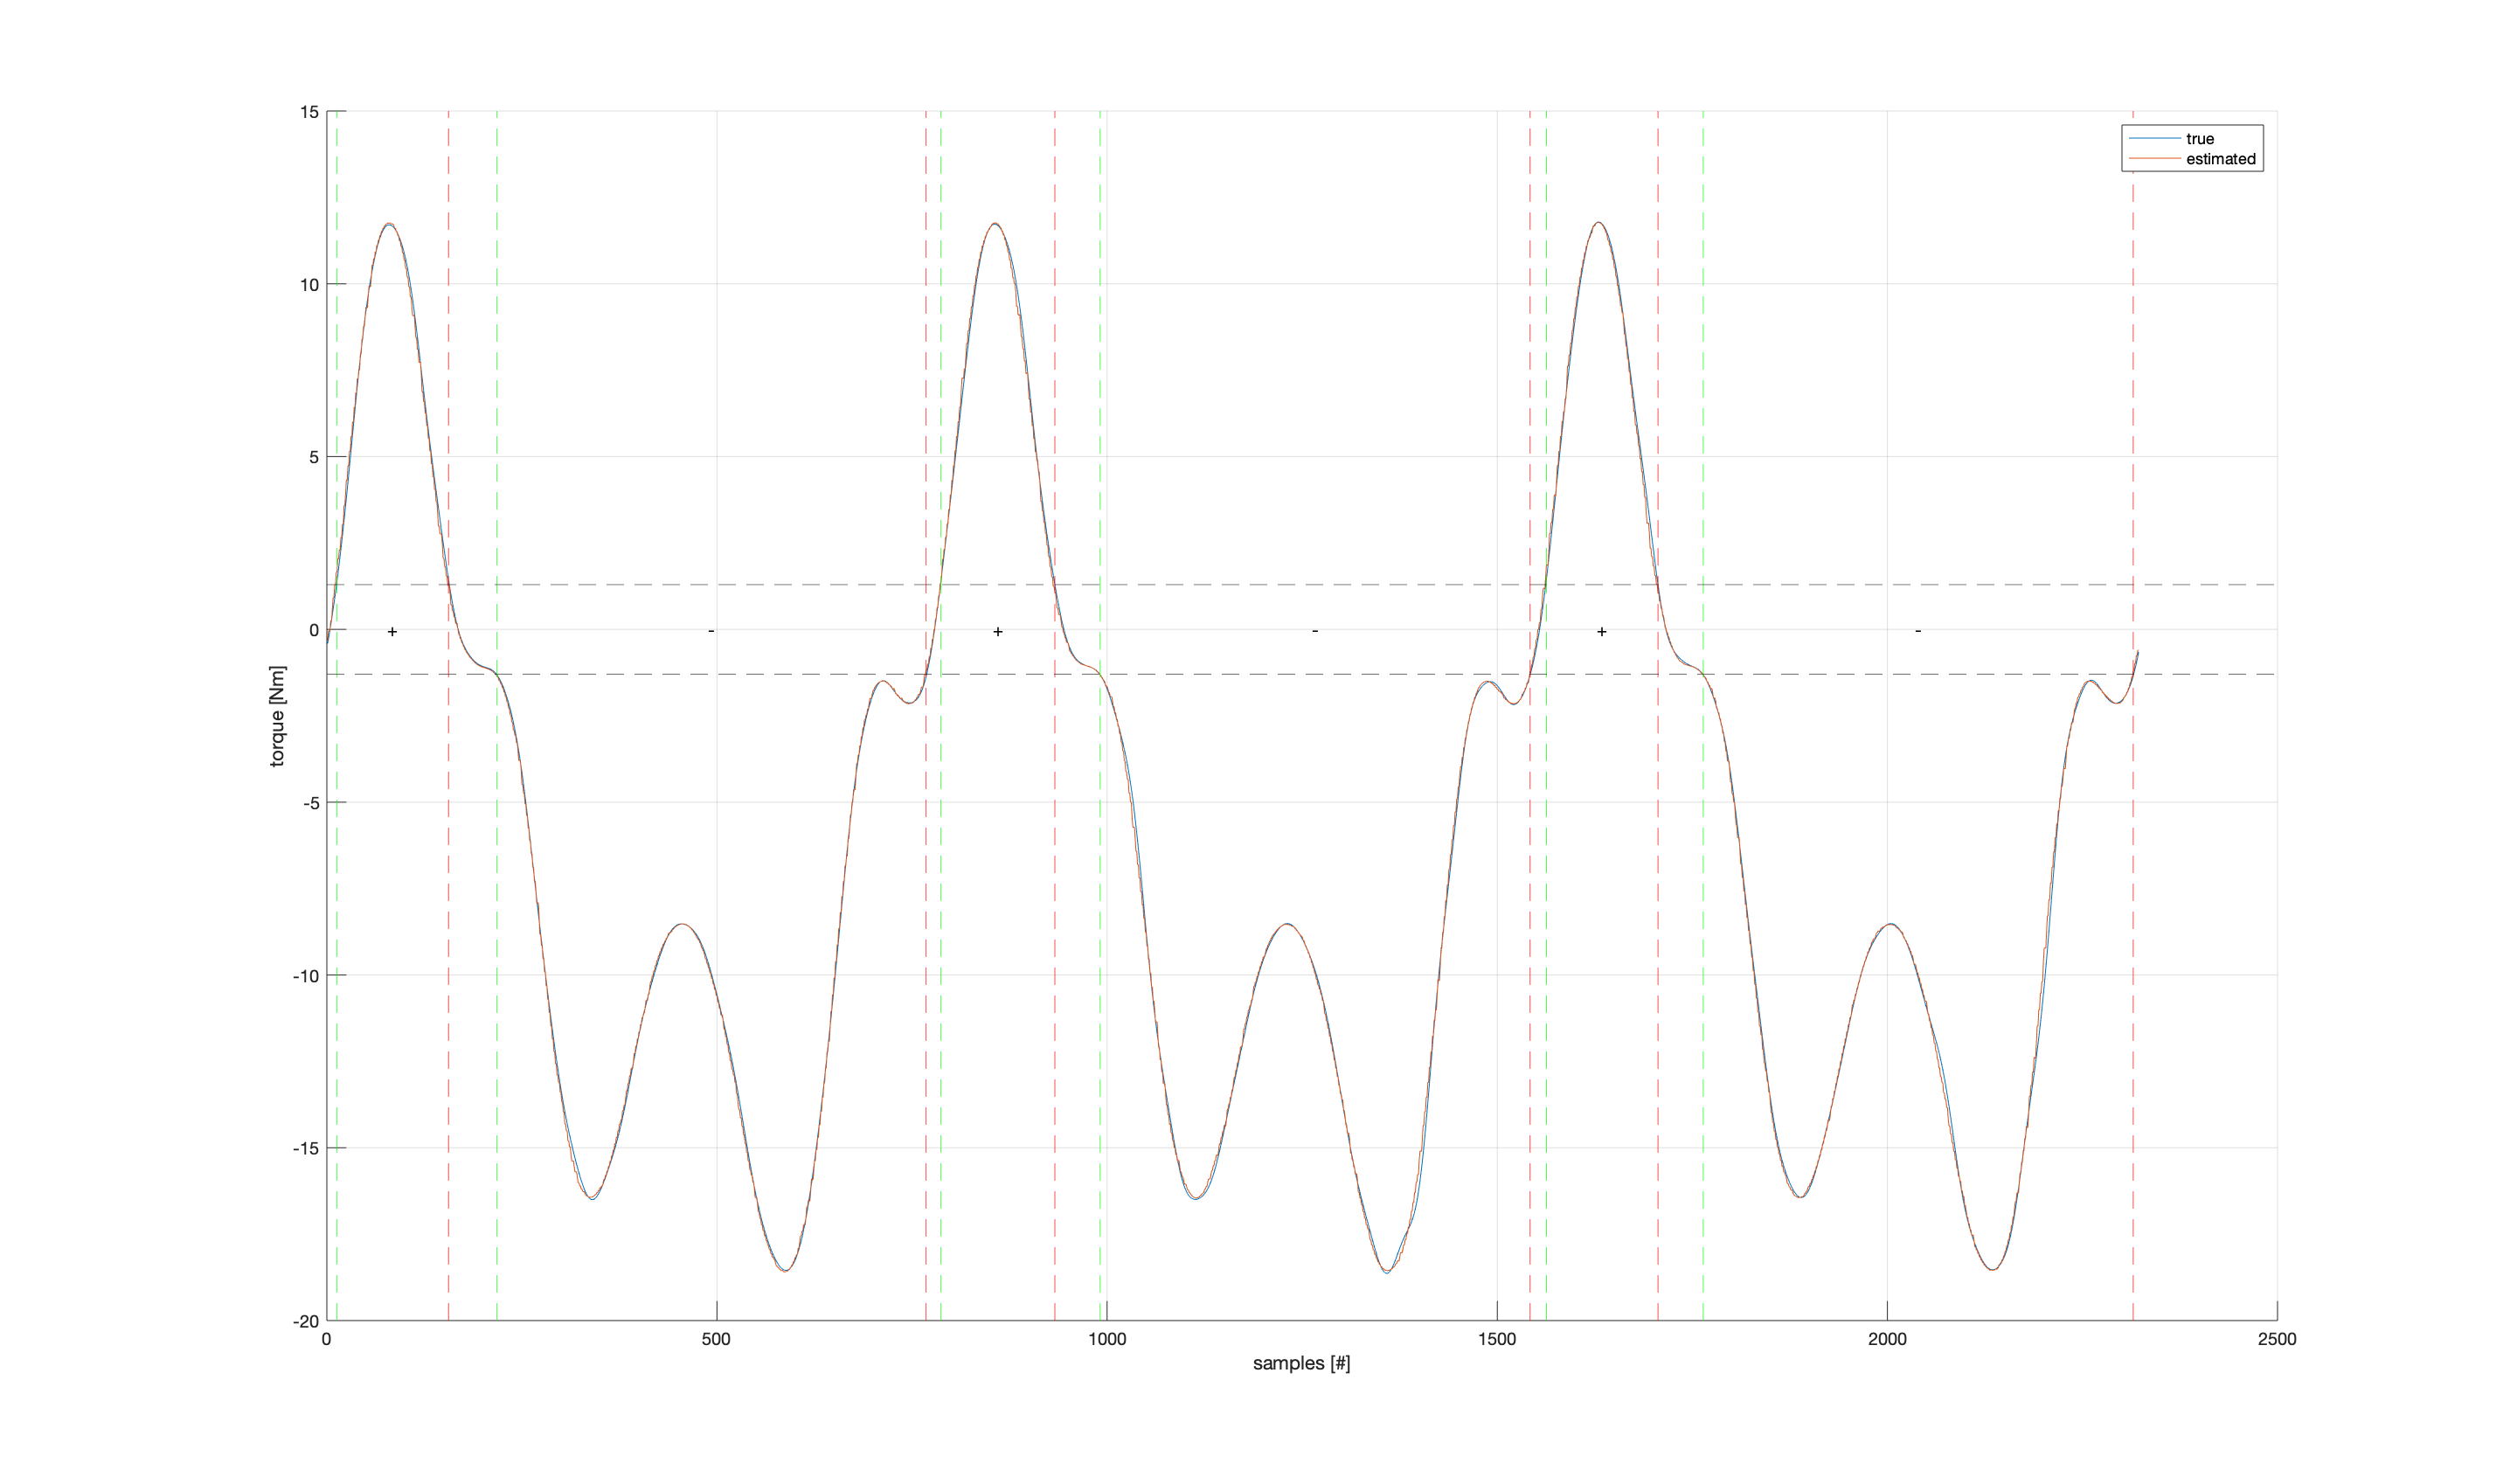
\includegraphics[width=0.8\textwidth]{images/1-dof/results_experiment1.png}
\caption{Plot of the reconstructed torque vs nominal torque. The gray dashed lines represent the threshold; the green dashed lines represent the start of the segment, while the red dashed lines represent the end of the segment. Samples under threshold are discarded. The signs estimated by the algorithm are reported for each segment.}
\end{figure}
\FloatBarrier

\paragraph{Experiment 2} The estimated dynamic coefficients without torque signs are:

\[\begin{bmatrix}
\pi_1  \\ \pi_2 
\end{bmatrix}=\begin{bmatrix}
24.4203 \\ 0.9547
\end{bmatrix}\]

The norm of the error is 0.7237.

\begin{figure}[!htbp]
\centering
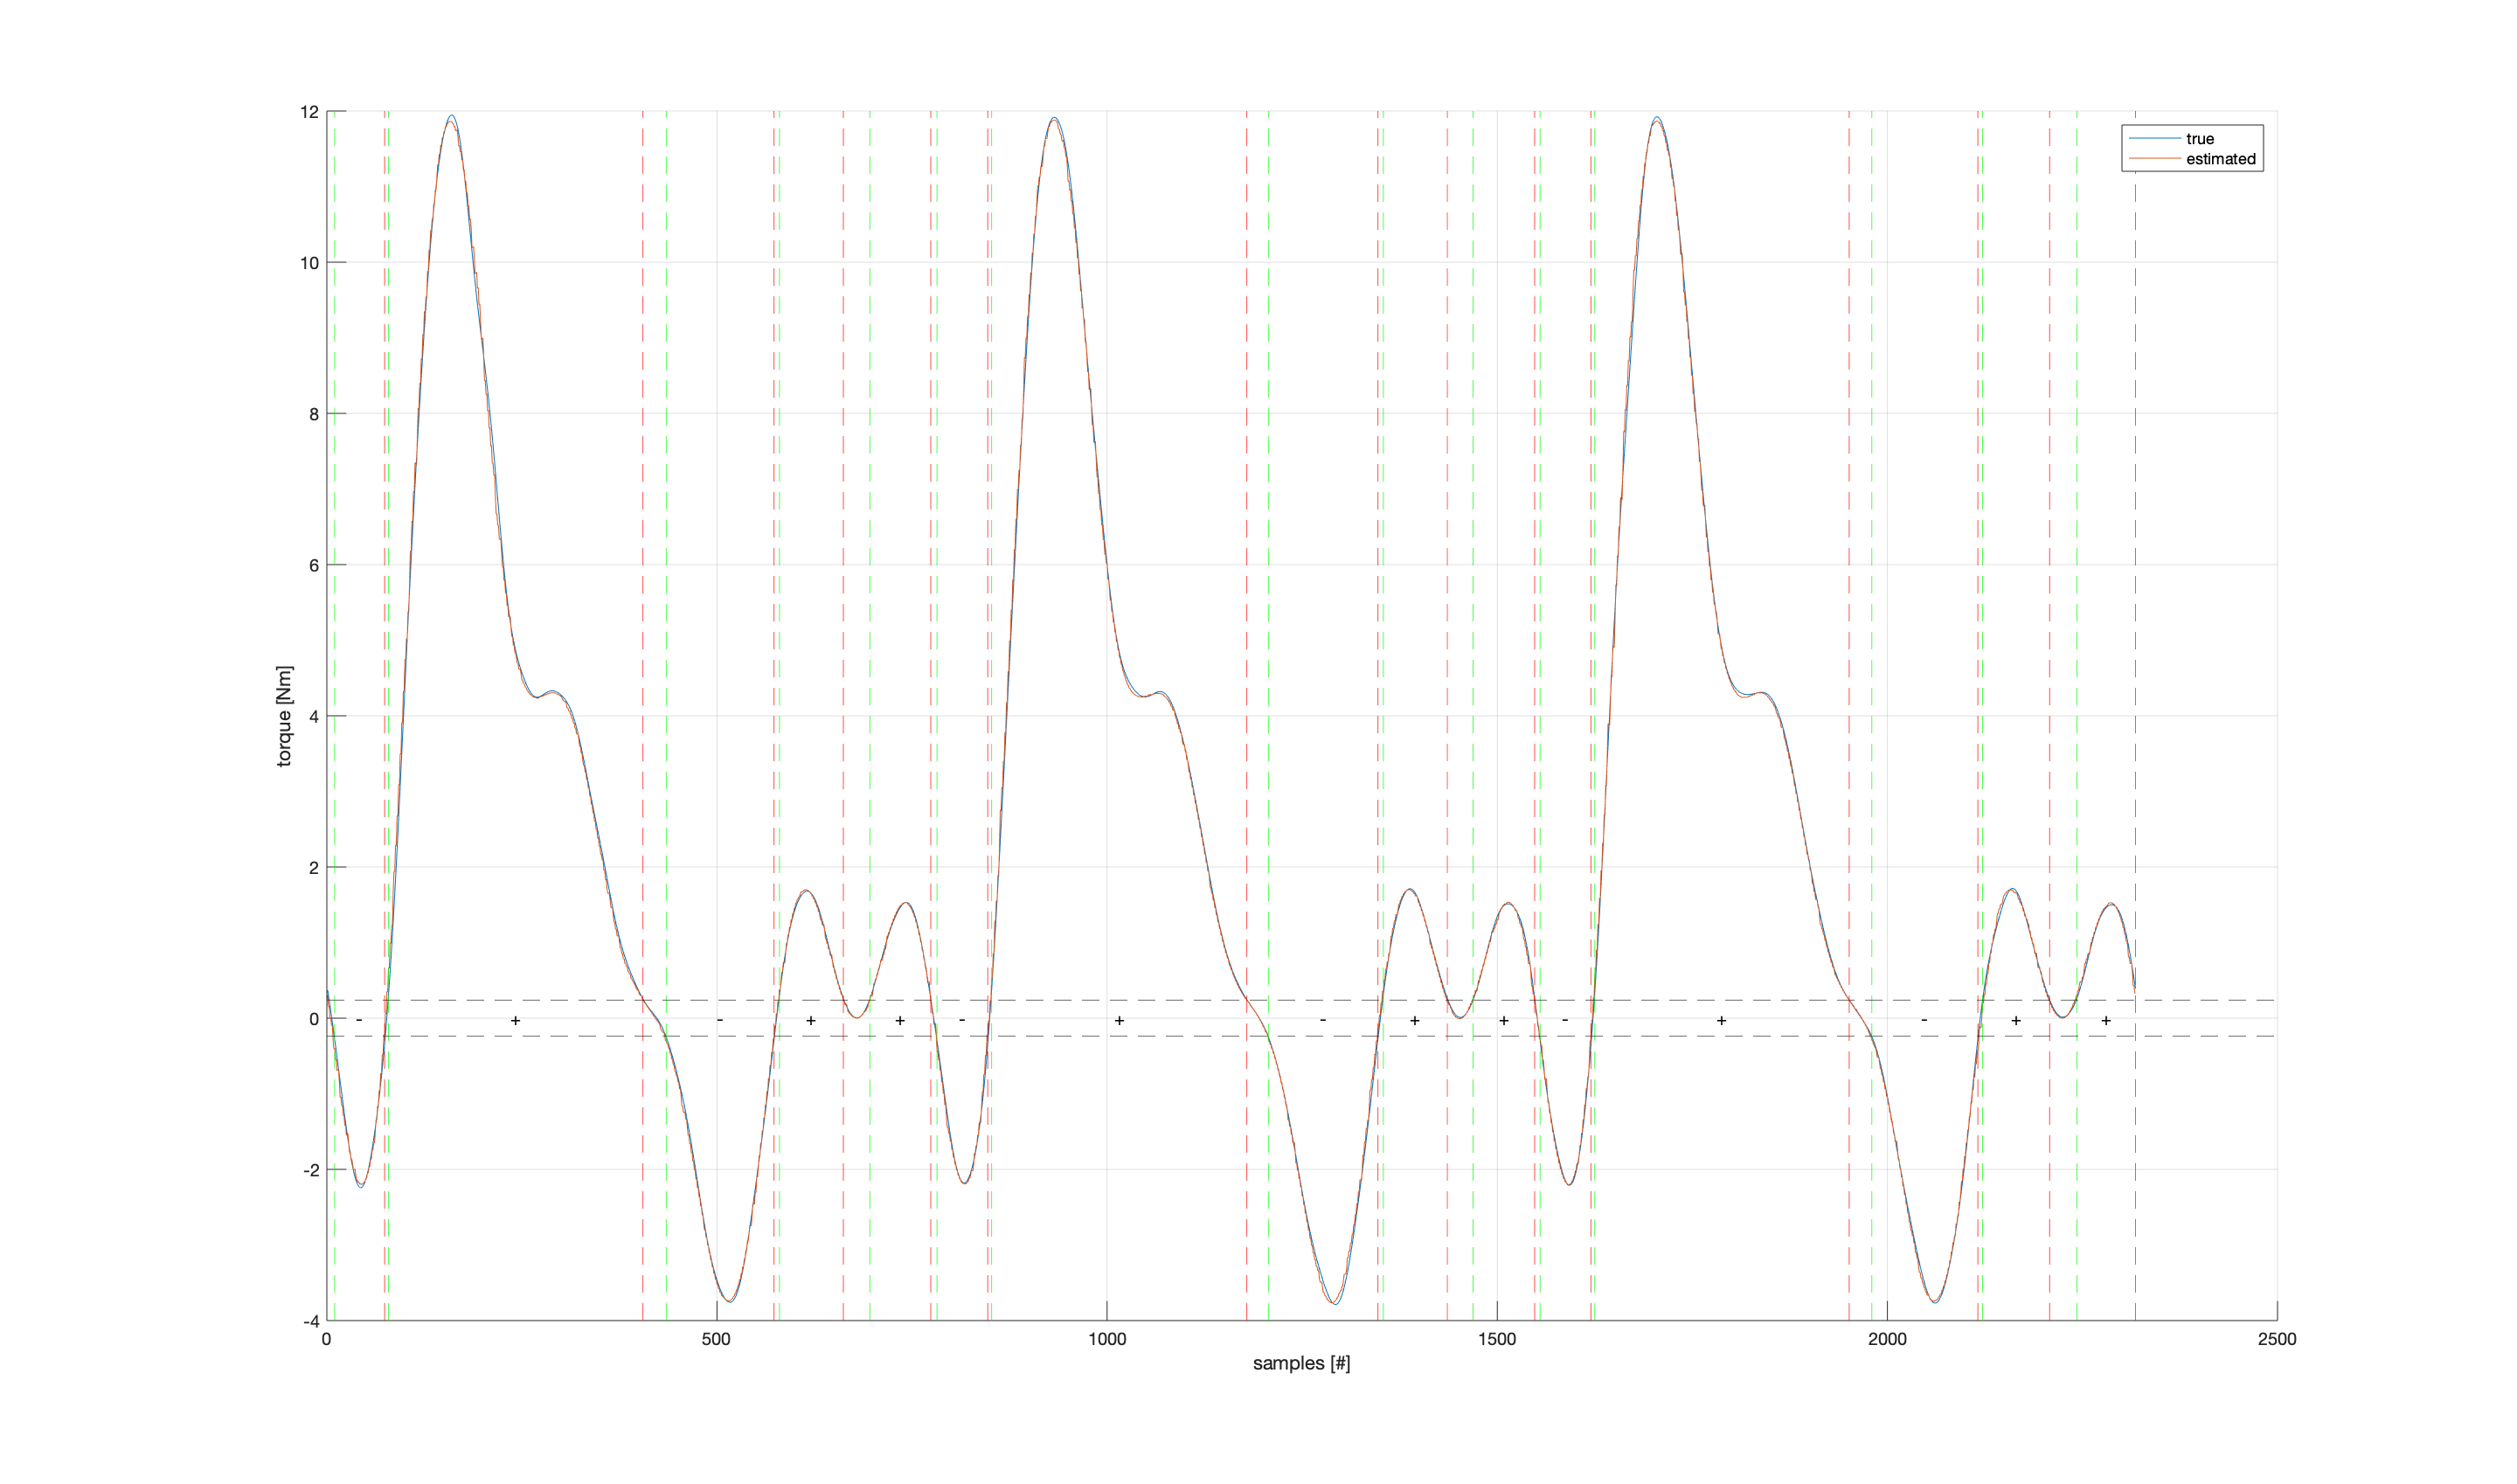
\includegraphics[width=0.8\textwidth]{images/1-dof/results_experiment2.png}
\caption{Plot of the reconstructed torque vs nominal torque. The gray dashed lines represent the threshold; the green dashed lines represent the start of the segment, while the red dashed lines represent the end of the segment. Samples under threshold are discarded. The signs estimated by the algorithm are reported for each segment.}
\end{figure}
\FloatBarrier

\paragraph{Experiment 3} The estimated dynamic coefficients without torque signs are:

\[\begin{bmatrix}
\pi_1  \\ \pi_2 
\end{bmatrix}=\begin{bmatrix}
24.5510 \\ 1.0367
\end{bmatrix}\]

The norm of the error is 0.6346.

\begin{figure}[!htbp]
\centering
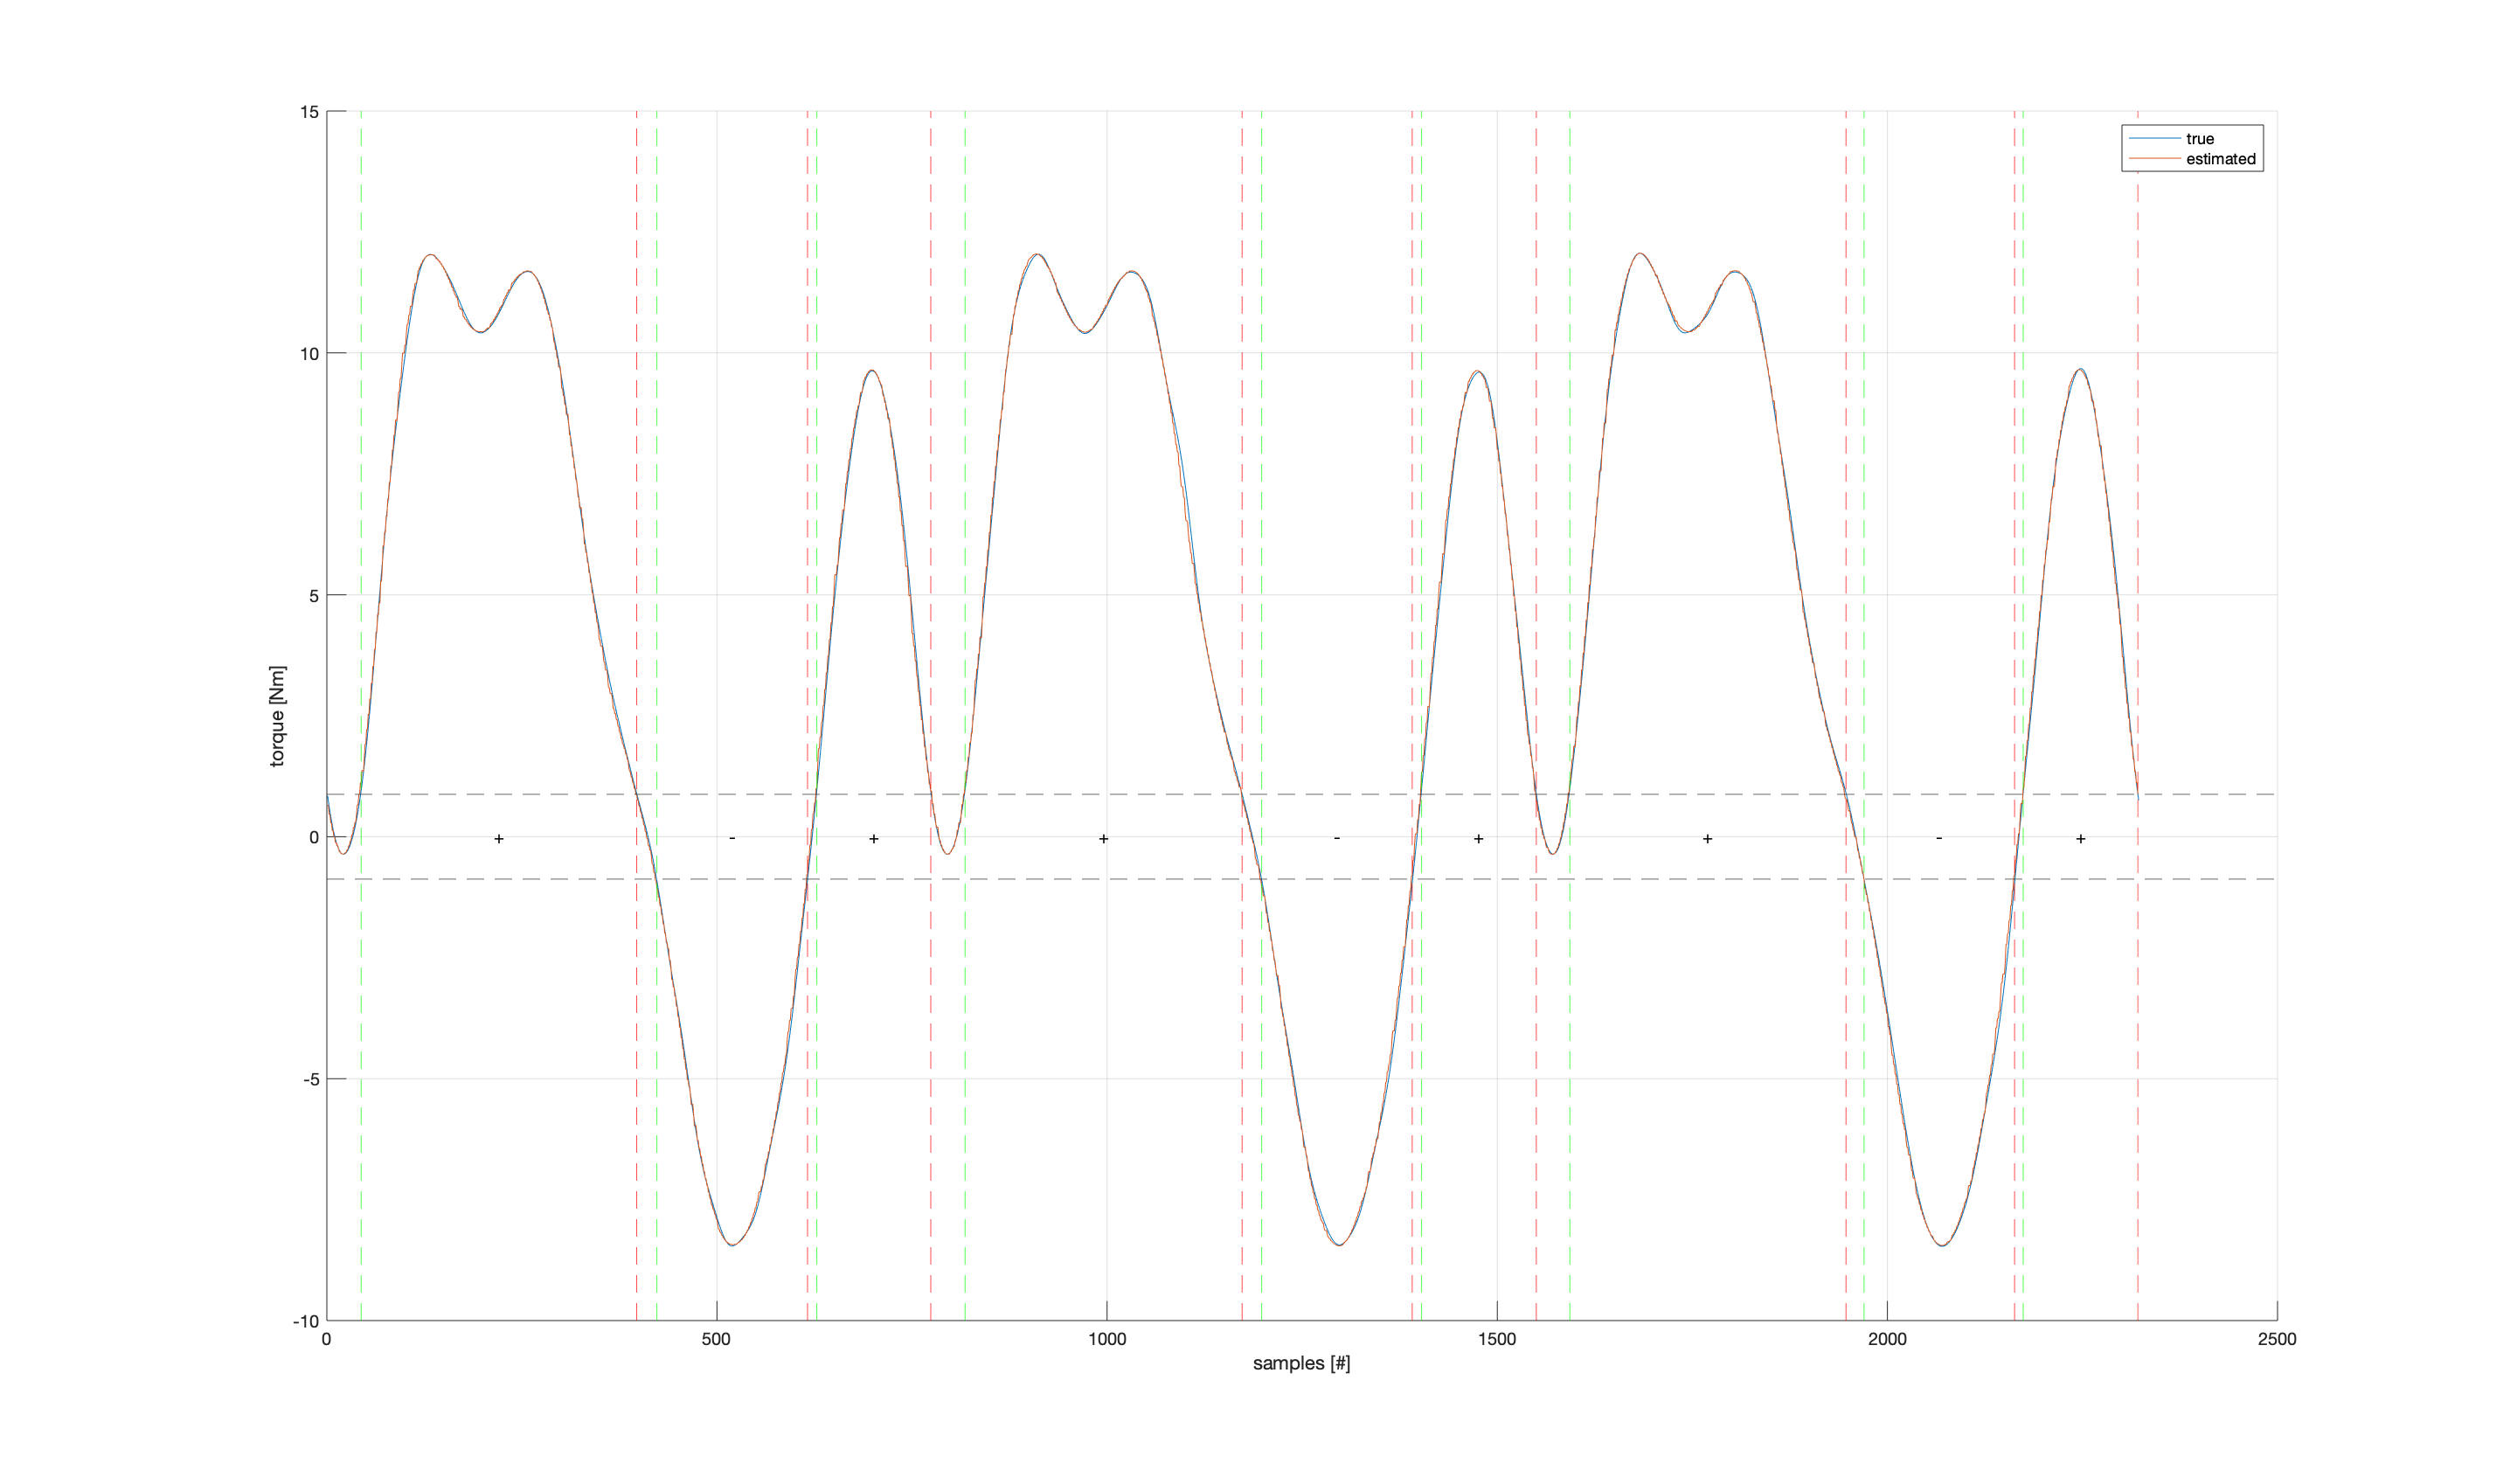
\includegraphics[width=0.8\textwidth]{images/1-dof/results_experiment3.png}
\caption{Plot of the reconstructed torque vs nominal torque. The gray dashed lines represent the threshold; the green dashed lines represent the start of the segment, while the red dashed lines represent the end of the segment. Samples under threshold are discarded. The signs estimated by the algorithm are reported for each segment.}
\end{figure}
\FloatBarrier

\paragraph{Experiment 4} The estimated dynamic coefficients without torque signs are:

\[\begin{bmatrix}
\pi_1  \\ \pi_2 
\end{bmatrix}=\begin{bmatrix}
24.5375 \\ 1.0094
\end{bmatrix}\]

The norm of the error is 0.6616.

\begin{figure}[!htbp]
\centering
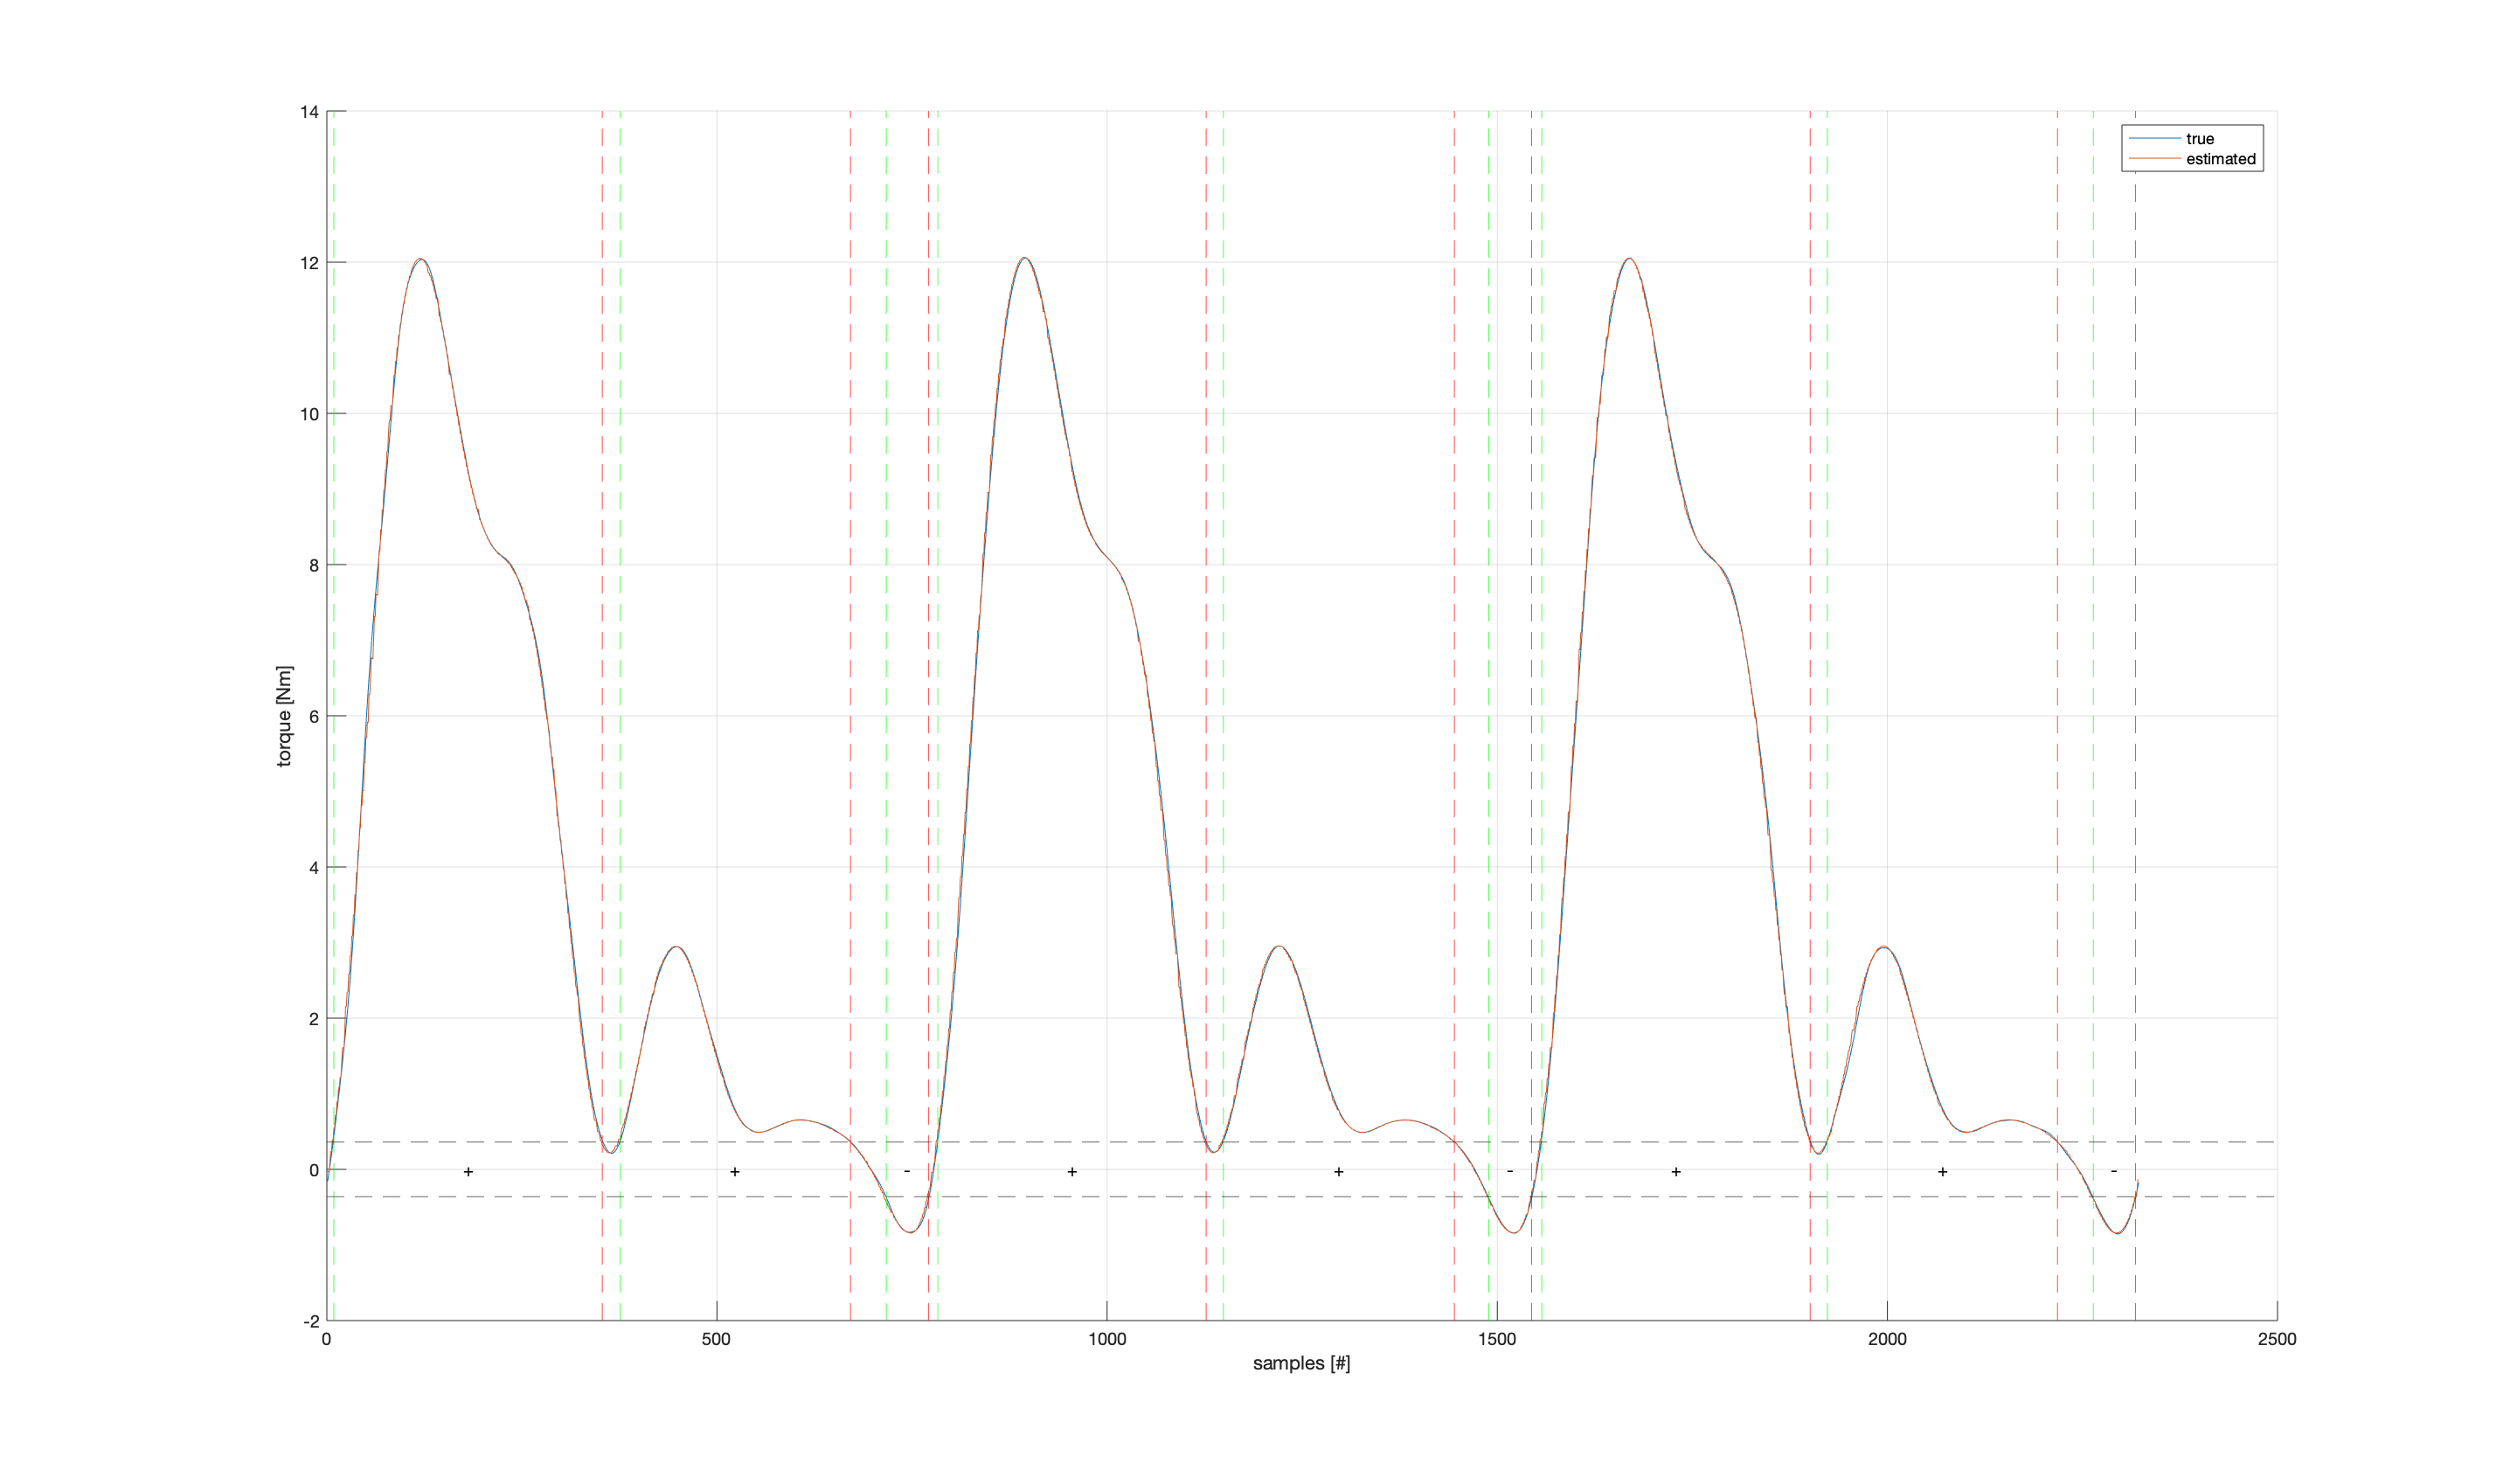
\includegraphics[width=0.8\textwidth]{images/1-dof/results_experiment4.png}
\caption{Plot of the reconstructed torque vs nominal torque. The gray dashed lines represent the threshold; the green dashed lines represent the start of the segment, while the red dashed lines represent the end of the segment. Samples under threshold are discarded. The signs estimated by the algorithm are reported for each segment.}
\end{figure}
\FloatBarrier

\section{3R spatial robot}
After the simple case, we tried to extend this procedure to a more complex robot: a 3R spatial robot.\\
So, first of all we needed to determine the structure of the robot by defining the Denavit-Hartenberg parameters and to determine the symbolic dynamic model of the robot.
\subsection{Robot structure}
\subsubsection*{Denavit-Hartenberg}
\paragraph{}
\FloatBarrier
\begin{table}[!htbp]
\centering
\begin{tabular}{|c|cccc|}
\hline
& $\alpha$ & a & d & $\theta$\\
\hline
link 1 & $\pi$/2 & 0 & $L_1=0.3$ & $q_1$\\
link 2 & 0 & $L_2=0.3$ & $-d_2=-0.09$ & $q_2$\\
link 3 & 0 & $L_3=0.2$ & 0 & $q_3$\\
\hline
\end{tabular}
\caption{In this table the DH parameters of the robot are reported.}
\end{table}
\subsubsection*{D-H Frames}

\begin{center}
\begin{figure}[!htb]
   \begin{minipage}{0.33\textwidth}
     \centering
     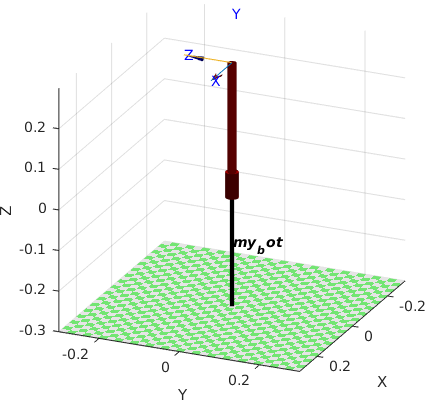
\includegraphics[width=\linewidth]{images/3-dof/frame1.png}
   \end{minipage}\hfill
   \begin{minipage}{0.33\textwidth}
     \centering
     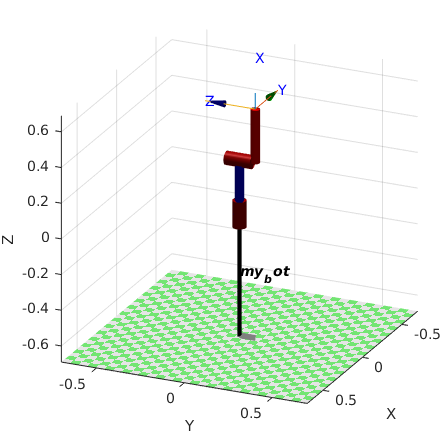
\includegraphics[width=\linewidth]{images/3-dof/frame2_q2_90.png}
   \end{minipage}\hfill
   \begin{minipage}{0.33\textwidth}
     \centering
     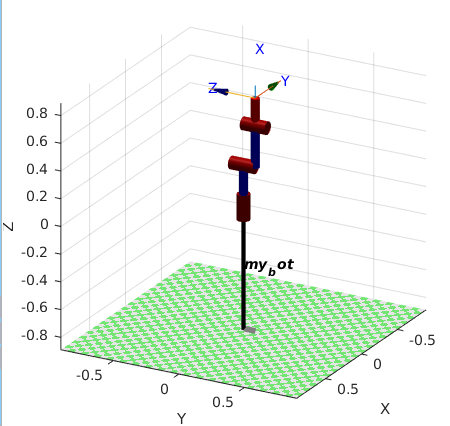
\includegraphics[width=\linewidth]{images/3-dof/frame3_q2_90.png}
   \end{minipage}
   \caption{(a) Frame 1 (b) Frame 2 (c) Frame 3}

\end{figure} 
\end{center}
\FloatBarrier

\subsubsection*{Centers of Mass}
We computed the position of the centers of mass in their respective frames, according to the DH frames we just defined.

\[r_{c1}=\begin{pmatrix}
0\\
-a\\
0\\
\end{pmatrix} = \begin{pmatrix}
0\\
-0.15\\
0\\
\end{pmatrix}
\]
\[r_{c2}=\begin{pmatrix}
-b\\
0\\
-c\\
\end{pmatrix} = \begin{pmatrix}
-0.15\\
0\\
-0.06\\
\end{pmatrix}
\]
\[r_{c3}=\begin{pmatrix}
-d\\
0\\
0\\
\end{pmatrix} = \begin{pmatrix}
-0.10\\
0\\
0\\
\end{pmatrix}
\]
%\[a=0.15;\qquad b=0.15;\qquad c=0.06;\qquad d=0.10 
%\]
\subsubsection*{Dynamic model}
To compute the dynamic model of the robot we followed these steps:
\begin{itemize}
\item We implemented the moving frame algorithm in order to obtain the linear and angular velocities of the frames origin;
\item We computed the kinetic energy expressing the inertial tensors with respect to the centers of mass;
\item From the kinetic energy, we computed the inertia matrix and the Coriolis and centrifugal terms of the model;
\item After that we computed the potential energy, using the centers of mass expressed with respect to the base frame and we computed the gravity vector.
\end{itemize}
Once we obtained the dynamic model of the robot, we found a minimal representation of the model. The dynamic coefficients we found are given by:

\[\pi_1= I_{1,yy} + m_2 (c+ d_2)^2 + m_3 d_2^2\]
\[\pi_2 = m_2(L_2 -b)^2 + m_3 L_2^2 + I_{2,yy}\]
\[\pi_3 = I_{2,xx}\]
\[\pi_4 = I_{3,yy} + m_3(L_3 - d)^2\]
\[\pi_5 = I_{3,xx}\]
\[\pi_6 = m_3(L_3 -d)L_2\]
\[\pi_7 = I_{2,zz} + m_2(L_2 - b)^2 + I_{3,zz} + m_3(L_2^2 + (L_3 - d)^2 )\]
\[\pi_8 = m_3(L_3 -d)^2 + I_{3,zz}\]
\[\pi_9 = m_2(L_2 - b)(c+ d_2) + m_3 L_2 d_2\]
\[\pi_{10} = m_3(L_3 - d)d_2\]
\[\pi_{11} = g_0 m_2 (L_2 - b)\]
\[\pi_{12} = g_0 m_3 (L_3 - d)\]
\[\pi_{13} = g_0 m_3 L_2\]
\subsection{Simulation}
We created a new V-REP scene from scratch, and we represented the robot arm we just discussed.
\FloatBarrier
\begin{figure}[!htbp]
\centering
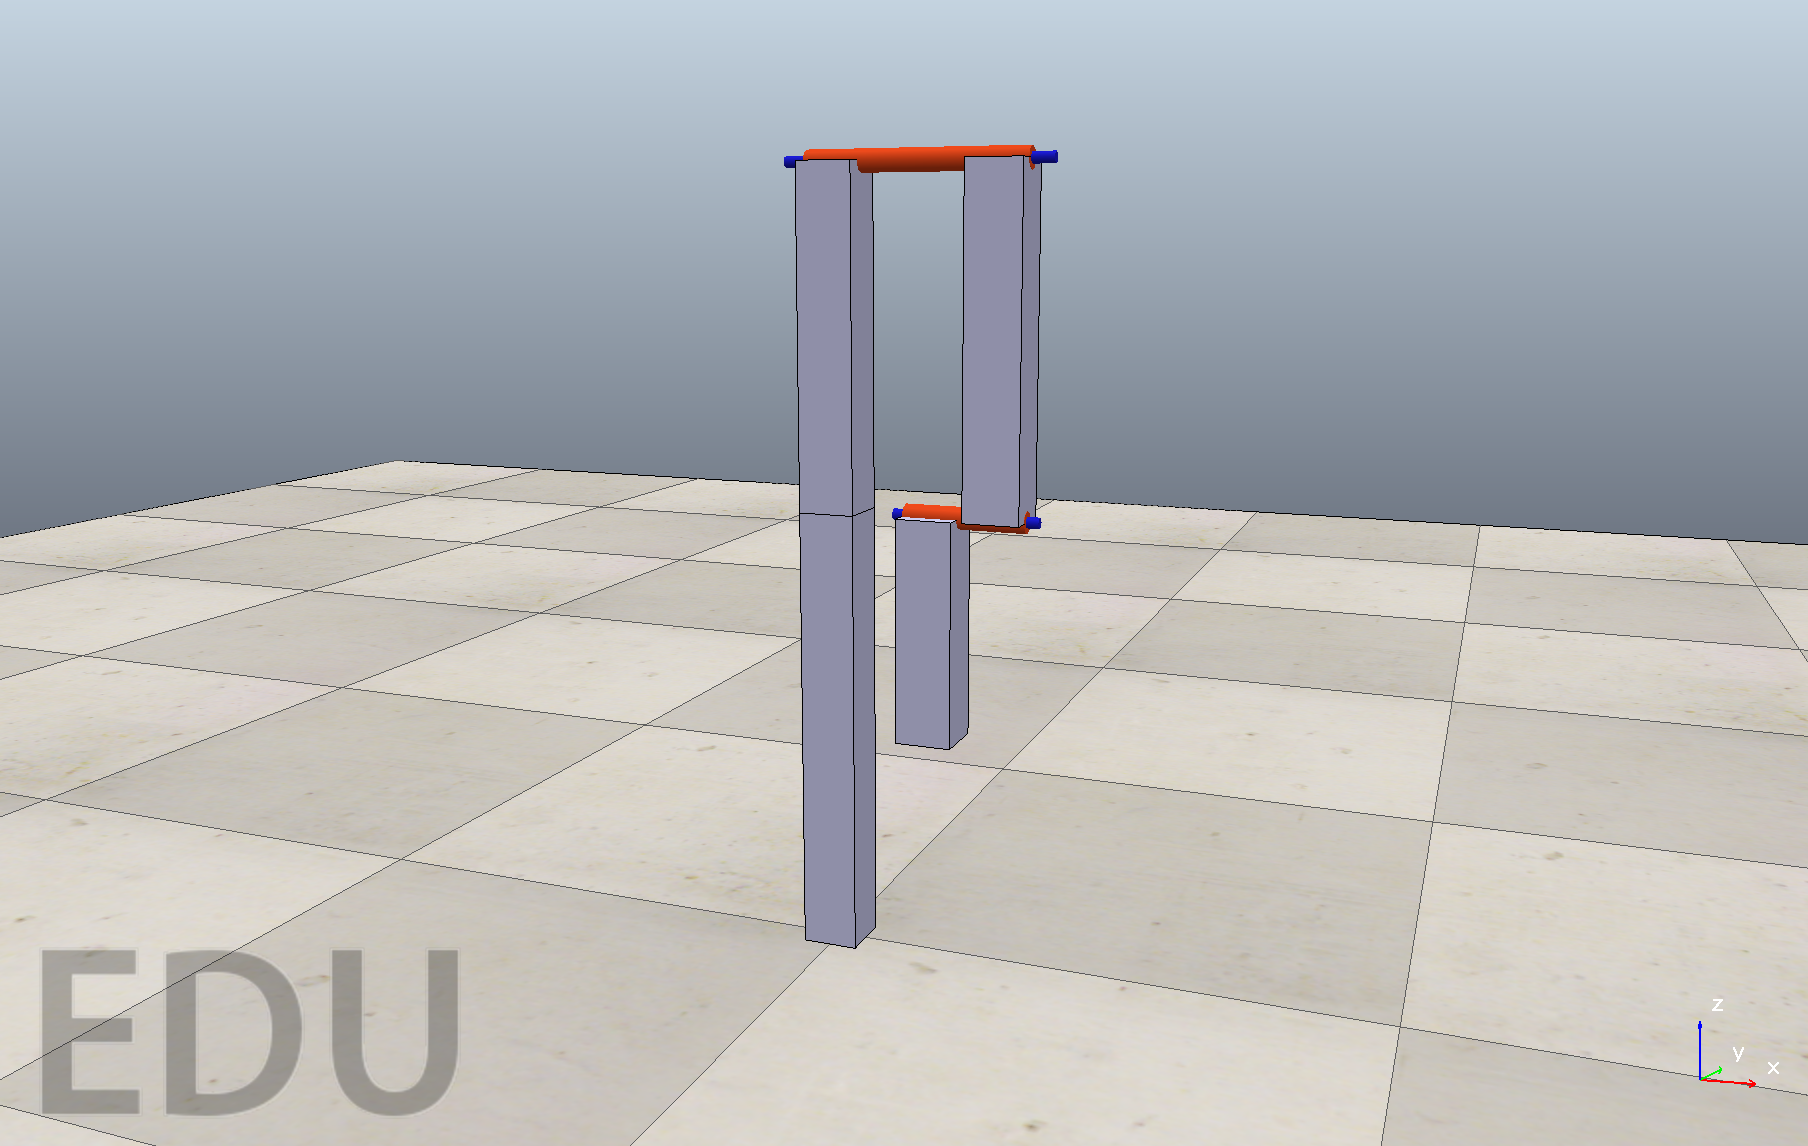
\includegraphics[width=0.7\textwidth]{images/3-dof/scene.png}
\caption{3R Robot-arm V-REP scene}
\end{figure}
\FloatBarrier
For the simulation we used the following values for masses and inertia tensors.
\[m_1 = 10 \;kg,\quad I_{xx,1} = 7.708\cdot 10^{-2}\;kg\cdot m^2,\quad I_{yy,1} = 4.167 \cdot 10^{-3}\;kg\cdot m^2,\quad I_{zz,1} = 7.708\cdot 10^{-2}\;kg\cdot m^2\]
\[ m_2 = 1.125\;kg,\quad I_{xx,2} = 4.6879\cdot10^{-4}\;kg\cdot m^2,\quad I_{yy,2} = 8.6715\cdot 10^{-3}\;kg\cdot m^2,\quad I_{zz,2} = 8.6715\cdot 10^{-3}\;kg\cdot m^2\]
\[m_3 = 0.75\;kg,\quad I_{xx,3} = 3.1252\cdot 10^{-4}\;kg\cdot m^2,\quad I_{yy,3} = 2.6565\cdot 10^{-3}\;kg\cdot m^2,\quad I_{zz,3} = 2.6565\cdot 10^{-3}\;kg\cdot m^2\]
The first and the second links are two parallelepipeds which length is 0.3 $m$ and their transversal section is a square with side equal to 0.05 $m$, while the third link is 0.2 $m$ long and has a transversal section that is a square with side equal to 0.05 $m$.\\\\
As reguards the simulation, we used the same approach of the 1R robot, but of course this time we had to deal with 3 links so we had 3 joint positions and 3 joint torques at each robot update.\\\\(vedi velocità)\\\\
We used Bullet2.78 as physics engine as we are interested in torque applied to the joint motor, and using this engine is the only way to get directly this information from the V-REP remote API.
\subsection{Experiments}
\subsection{PBRP algorithm}
We have extended the procedure for the 1R robot to the 3R case. Since we have more than one joint, we need to add some constraints; this is the complete algorithm:
\FloatBarrier
\begin{figure}[!htbp]
\centering
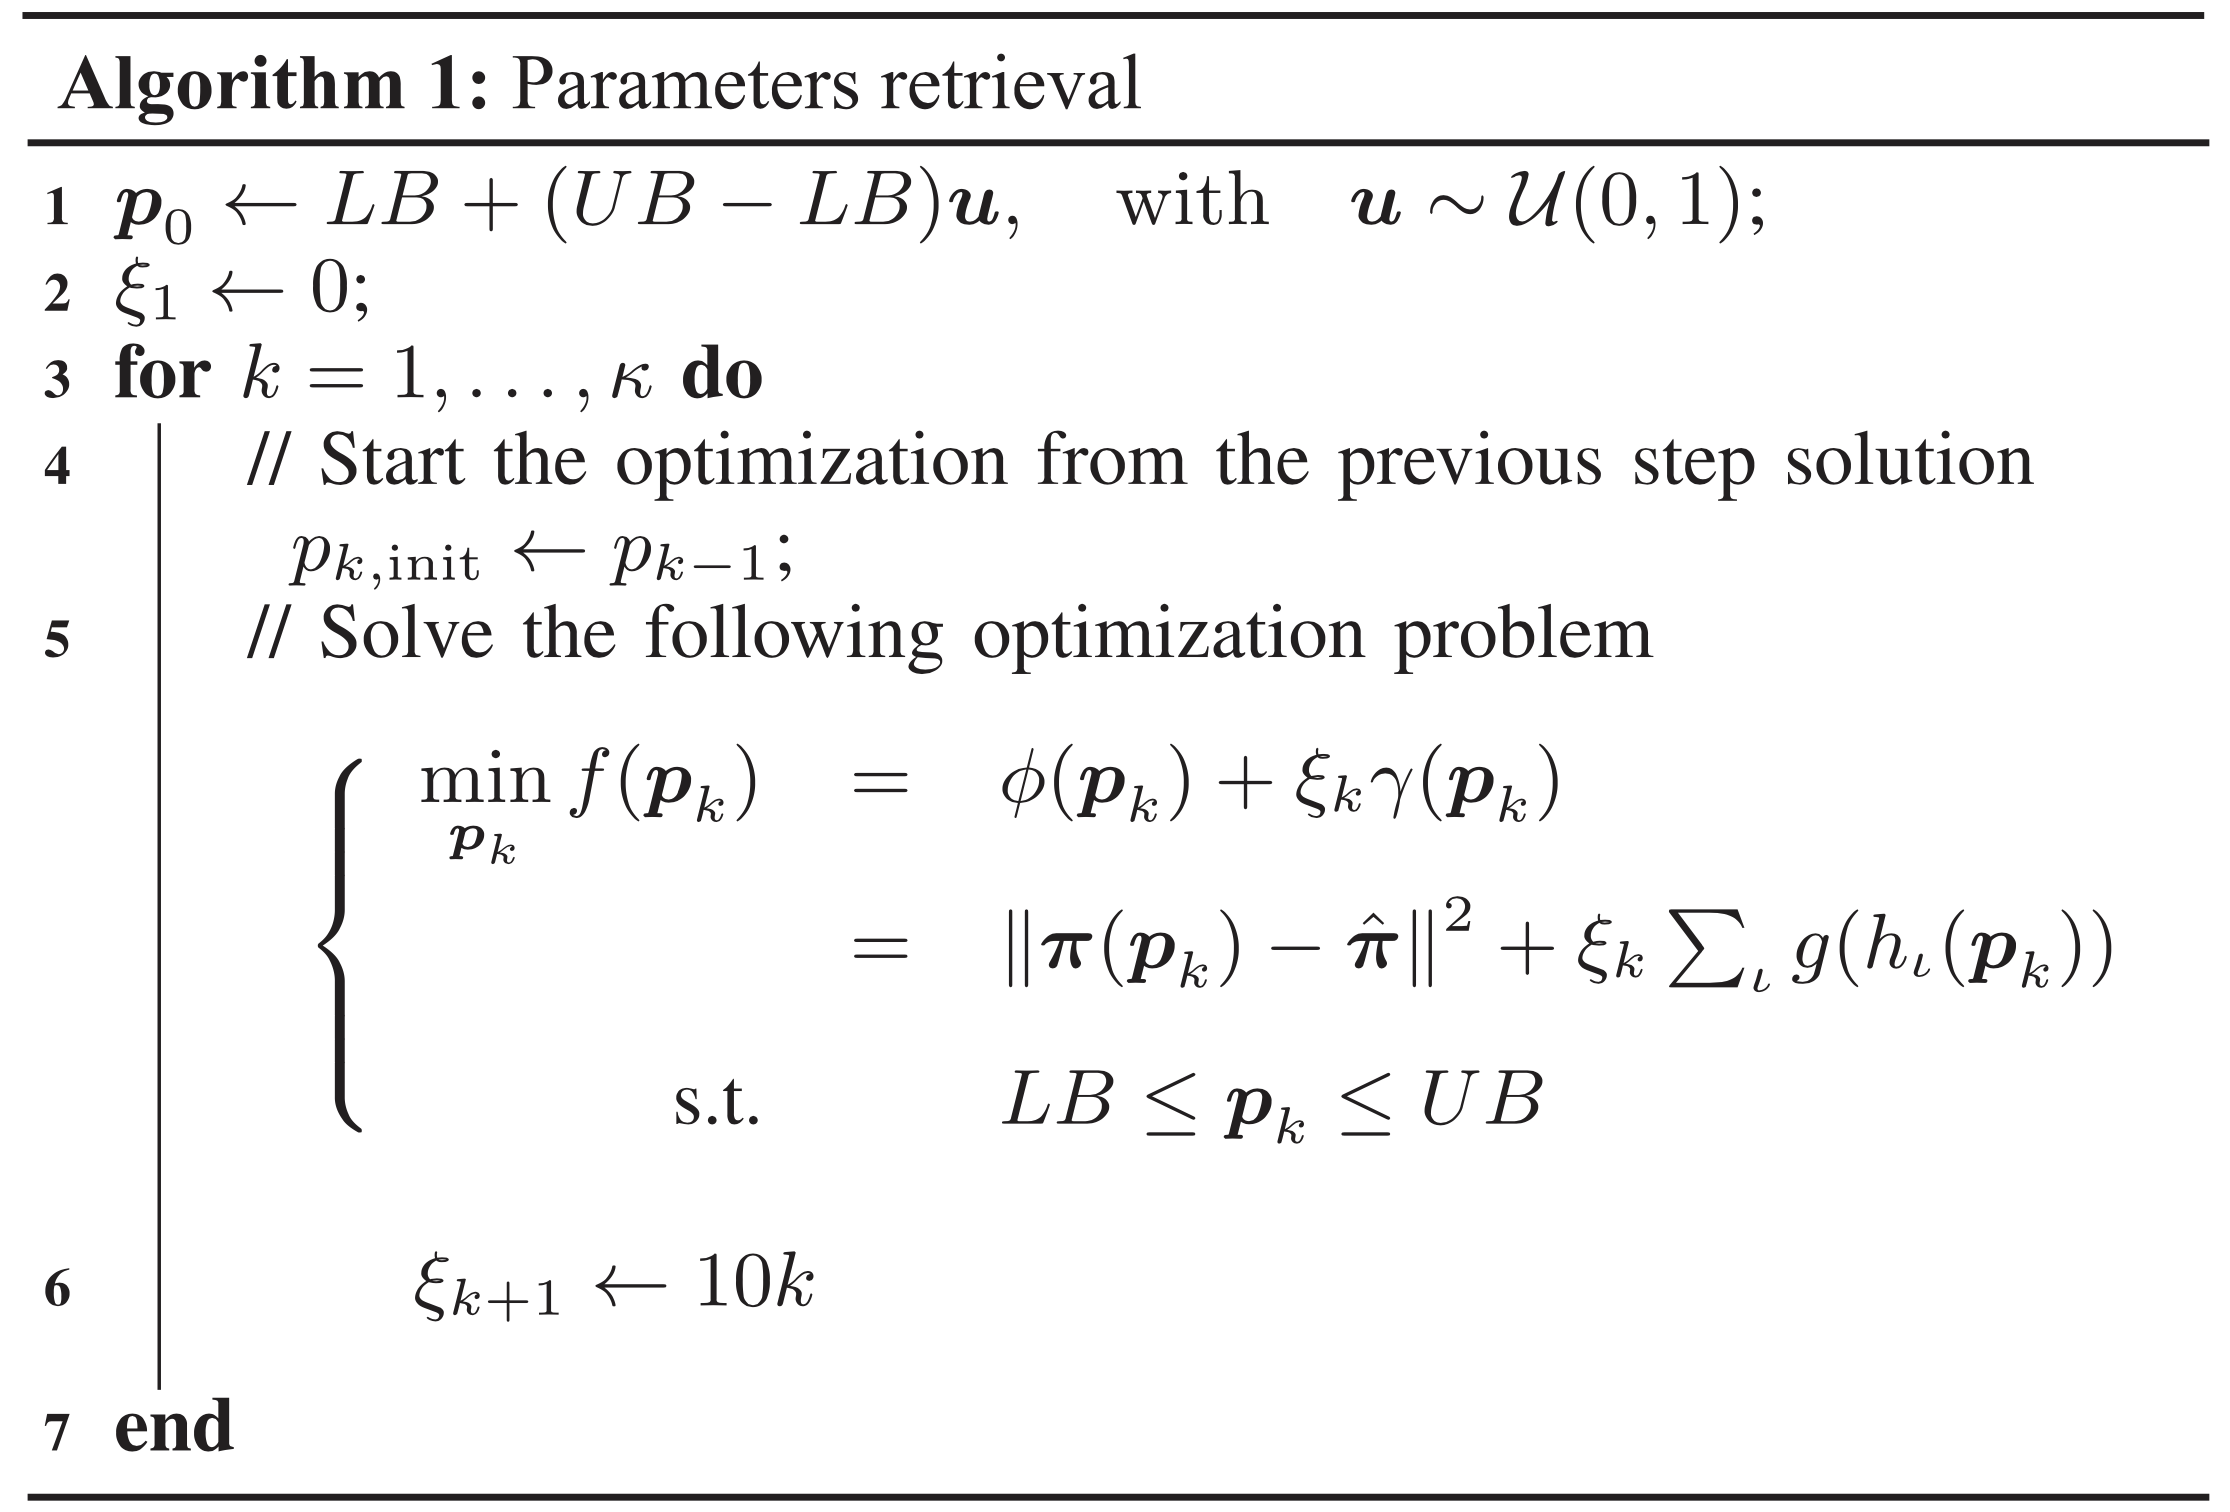
\includegraphics[width=0.6\textwidth]{images/3-dof/algorithm.png}
\caption{PBRP algorithm}
\end{figure}
\FloatBarrier
In particular, in addition to the lower and upper bounds,  for each link $l_i$ the following triangle inequalities regarding the inertias  must be satisfied:

\[\begin{cases}
\overline{I}_{i,x}+\overline{I}_{i,y} > \overline{I}_{i,z} \\
\overline{I}_{i,z}+\overline{I}_{i,y} > \overline{I}_{i,x} \\
\overline{I}_{i,x}+\overline{I}_{i,z} > \overline{I}_{i,y}
\end{cases}\]

These inequalities can be rewritten as:

\[\frac{tr(I_{l_i})}{2}-\lambda_{max}(I_{l_i})>0\]

Moeover, the total sum of the link masses must be in a given range, that is:

\[m_{rob,min}\le \sum_i{m_i} \le m_{rob,max}\]

The search algorithm is simulated annealing as before and we run the algorithm 3 times.
\subsection{Tree of solutions}
The tree algorithm is a simple extension of the 1R case; we highlight the fact that segments of different links are put and examinated together in random order, so that we do not give priority to any link or segment. The algorithm used to solve the optimization problems of the tree is pattern search like in the previous case.
\\\\
After the tree has been built, we have the sequence of most likely signs that we apply to the absolute torques. Finally, we run the PBRP algorithm to the torques with the estimated signs for 3 times by using simulated annealing as search algorithm.
\subsection{Results}
\section{Conclusions}



\end{document}